% arara: pdflatex: { synctex: yes }
% arara: makeindex: { style: ctuthesis }
%% arara: bibtex

%\listfiles


%\PassOptionsToPackage{cp1250}{inputenc}

% The class takes all the key=value arguments that \ctusetup does,
% and couple more: draft and oneside
\documentclass[twoside]{ctuthesis}

\makeatletter
\edef\mytoday{\expandafter\@gobbletwo\the\year\ifnum\month<10 0\fi\the\month\ifnum\day<10 0\fi\the\day}
\makeatother

% LaTeX logo with better kerning in sf bf font
\makeatletter
\newcommand\LaTeX@lmss@bx{L\kern -.33em{\sbox \z@ T\vbox to\ht \z@ {\hbox {\check@mathfonts \fontsize \sf@size \z@ \math@fontsfalse \selectfont A}\vss }}\kern -.15em\TeX}
\DeclareRobustCommand\myLaTeX{%
	\ifcsname LaTeX@\f@family @\f@series\endcsname
		\csname LaTeX@\f@family @\f@series\endcsname
	\else
		\LaTeX
	\fi
}

\usepackage{datetime}
\ctusetup{
%	preprint = {\ctuverlog \\ ctuman \mytoday},
	mainlanguage = english,
	titlelanguage = english,
	otherlanguages = {english, czech},
	title-czech = {Hluboké neuronové sítě ve vestavěných systémech},
	title-english = {Deep Neural Networks in Embedded Systems},
	doctype-czech = {Diplomová práce},
	doctype-english = {Master's Thesis},
	xfaculty = F3,
	department-czech = {Katedra kybernetiky},
	department-english = {Department of Cybernetics},
	author = {Bc. Mykhaylo Zelenskyy},
	supervisor = {Ing. Lukáš Hrubý},
%	supervisor-address = {Ústav X, \\ Uliční 5, \\ Praha 99},
	keywords-czech = {},
	keywords-english = {},
	day = \the\day,
	month = \the\month,
	year = \the\year,
%	list-of-figures = false,
%	list-of-tables = false,
%	monochrome = true,
%	savetoner = true,
	pkg-listings = true,
	ctulstbg = none,
%	layout-short = true,
%	pkg-hyperref = false,
}

\ctuprocess

% Theorem declarations, this is the reasonable default, anybody can do what they wish.
% If you prefer theorems in italics rather than slanted, use \theoremstyle{plainit}
\theoremstyle{plain}
\newtheorem{theorem}{Theorem}[chapter]
\newtheorem{corollary}[theorem]{Corollary}
\newtheorem{lemma}[theorem]{Lemma}
\newtheorem{proposition}[theorem]{Proposition}

\theoremstyle{definition}
\newtheorem{definition}[theorem]{Definition}
\newtheorem{example}[theorem]{Example}
\newtheorem{conjecture}[theorem]{Conjecture}

\theoremstyle{note}
\newtheorem*{remark*}{Remark}
\newtheorem{remark}[theorem]{Remark}

\DeclareMathOperator{\atantwo}{atan2}

% Marginpars used as navigation aids.
%\PassOptionsToPackage{table,xcdraw}{xcolor}
\usepackage{colortbl}
\usepackage{tikz}

\usepackage{mparhack}
\usepackage{epstopdf}
\usepackage{subfig}
\usepackage{siunitx}
\usepackage{url}
\usepackage{multirow}
\usepackage[justification=centering]{caption}
\usepackage{amsmath}
\usepackage[framemethod=tikz]{mdframed}
\usepackage{url}
\usepackage{hyperref}
%\usepackage{degrade}

\usepackage{graphicx}

\usepackage{hhline}

\usepackage[edges]{forest}


\usepackage{textcomp}
\newcommand{\norm}[1]{\left\lVert#1\right\rVert}


\definecolor{folderbg}{RGB}{124,166,198}
\definecolor{folderborder}{RGB}{110,144,169}
\definecolor{foldercolor}{RGB}{124,166,198}

\def\Size{4pt}
\tikzset{pics/folder/.style={code={%
			\node[inner sep=0pt, minimum size=#1](-foldericon){};
			\node[folder style, inner sep=0pt, minimum width=0.3*#1, minimum height=0.6*#1, above right, xshift=0.05*#1] at (-foldericon.west){};
			\node[folder style, inner sep=0pt, minimum size=#1] at (-foldericon.center){};}
	},
	pics/folder/.default={20pt},
	folder style/.style={draw=foldercolor!80!black,top color=foldercolor!40,bottom color=foldercolor}
}

\forestset{is file/.style={edge path'/.expanded={%
			([xshift=\forestregister{folder indent}]!u.parent anchor) |- (.child anchor)},
		inner sep=1pt},
	this folder size/.style={edge path'/.expanded={%
			([xshift=\forestregister{folder indent}]!u.parent anchor) |- (.child anchor) pic[solid]{folder=#1}}, inner xsep=0.6*#1},
	folder tree indent/.style={before computing xy={l=#1}},
	folder icons/.style={folder, this folder size=#1, folder tree indent=3*#1},
	folder icons/.default={12pt},
}


\newcommand\indexmp[1]{{\sffamily\bfseries#1}}

\ExplSyntaxOn
\cs_new:Nn \ctuman_domarginpar:n {
	\marginpar
	[ \raggedleft \footnotesize \sffamily #1 ]
	{ \raggedright \footnotesize \sffamily #1 }
}
\cs_generate_variant:Nn \ctuman_domarginpar:n { x }
\DeclareDocumentCommand \ctump { m } {
	\clist_set:Nn \ctuman_temp_clist { #1 }
	\ctuman_domarginpar:x { \clist_use:Nnnn \ctuman_temp_clist { \\ } { \\ } { \\ } }
	\clist_map_inline:Nn \ctuman_temp_clist { \index{##1|indexmp} }
	\ignorespaces
}
\ExplSyntaxOff

% Abstract in Czech
\begin{abstract-czech}

\end{abstract-czech}

% Abstract in English
\begin{abstract-english}

\end{abstract-english}

% Acknowledgements / Podekovani
\begin{thanks}

\end{thanks}

% Declaration / Prohlaseni
\begin{declaration}
I declare that this work is all my own work and I have cited all sources I have
used in the bibliography.

\medskip

Prague, \monthinlanguage{second} \ctufield{day}, \ctufield{year}

\vspace*{2cm}

Prohlašuji, že jsem předloženou práci vypracoval samostatně, a že jsem uvedl veškerou použitou literaturu.

\medskip

V Praze, \ctufield{day}.~\monthinlanguage{title}~\ctufield{year}
\end{declaration}

\usepackage{url}

\usepackage{tabularx,array}

\usepackage{mathtools,amssymb}

% A savebox for typesetting listings in the titles
\newsavebox{\myboxa}

%\newcommand*\symbO{$\color{red}\bowtie$}
\newcommand*\symbO{\raisebox{0.5\height}{\scalebox{0.7}{\color{red}${\vartriangleright}\mkern-6mu{\vartriangleleft}$}}}
\newcommand*\symbM{\raisebox{0.5\height}{\scalebox{0.7}{\color{red}${\blacktriangleright}\mkern-6mu{\blacktriangleleft}$}}}
\newcommand*\itemO{\item\leavevmode\kern-0.33em\symbO}
\newcommand*\itemM{\item\leavevmode\kern-0.33em\symbM}



\begin{document}



% We actually don't want inline listings to have a background color
\renewcommand \ctulstsep {0pt}

% \ctuclsname for typesetting the class' name
\newcommand\ctuclsname{\leavevmode\unhcopy\ctuclsnamebox}
\newsavebox\ctuclsnamebox
\begin{lrbox}{\ctuclsnamebox}
\ctulst!ctuthesis!
\end{lrbox}

\maketitle

\chapter{Introduction}
\section{Nvidia Jetson}

Nvidia Jetson is a series of embedded modules producing by Nvidia designed for accelerating machine learning applications. First board, Jetson TK1, was presented in 2014. Jetson TK2 was announced in 2017  and was designed for low power systems like smaller camera drones. The next module called Jetson Xavier introduced in 2018 brings up to 20$\times$ acceleration compared to predecessor devises with power efficiency being improved 10$\times$. The newest Nvidia Nano was announced in 2019 and is focused on hobbyist robotics thanks to its low price. The last three modules are compared in \ref{jetson_comparison}.

\begin{figure}[h]
\caption{Nvidia Jetson comparison https://www.nvidia.com/en-us/autonomous-machines/embedded-systems/}
\label{jetson_comparison}
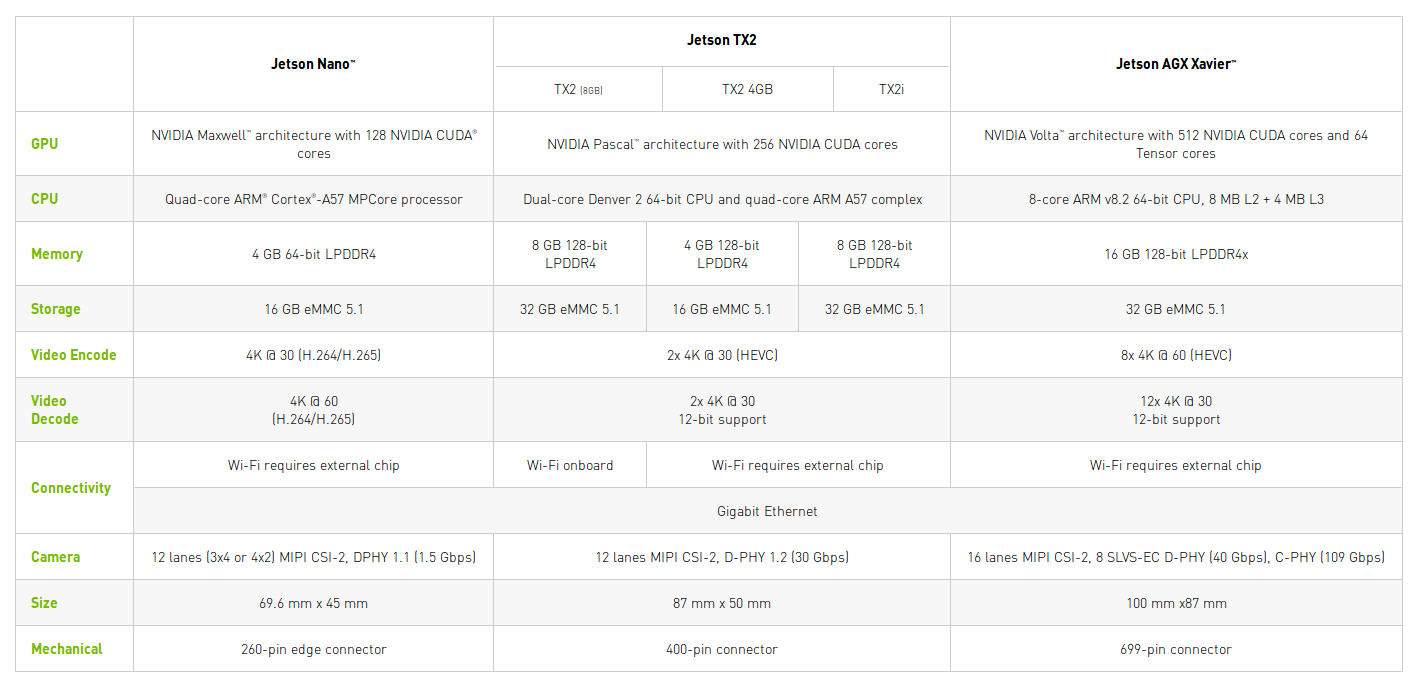
\includegraphics[width=\textwidth]{images/introduction/compare_jetson.png}
\end{figure}

As we can see, unlike other boards Jetson Xavier is build around NVIDIA Volta\texttrademark GPU with tensor cores. These tensor cores accelerate large matrix operations and can perform mixed-precision matrix multiplication and accumulate calculation in a single operation. Each core  provides a 4$\times$4$\times$4 matrix processing array which performs the operation $D = A \cdot B+C$ shown in \ref{tensor_core}, where $A,B,C,D$ are 4$\times$4 matrices. This operation is crucial for most of machine learning applications, especially in deep learning, because, as we will discuss in further chapters, output of each neuron in neural networks are calculated in similar way. 


\begin{figure}[h]
\caption{Tensor core operation https://devblogs.nvidia.com/programming-tensor-cores-cuda-9/}
\label{tensor_core}
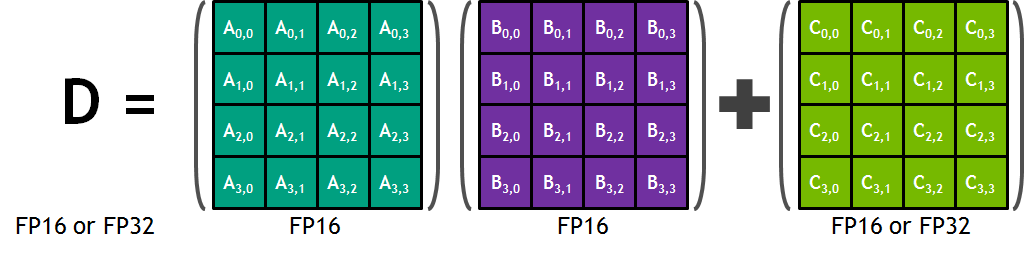
\includegraphics[width=\textwidth]{images/introduction/tensor_core.png}
\end{figure}

Another advantage of Jetson Xavier is using of Nvidia Deep Learning Accelerator engines http://nvdla.org/. These engines improve energy efficiency and free up the GPU to run more complex networks and implemented dynamic tasks  and has up to 5 trillion operations per second (TOPS) INT8 or 2.5 TFLOPS FP16 performance with a power consumption of only 0.5-1.5W. They also supports accelerating of CNN convolution, deconvolution, activation functions, min/max/mean pooling, local response normalization, and fully-connected layers.


\chapter{Related works}
\chapter{Neural networks}
Artificial neural networks are systems inspired by a brain.	The basic computation unit in a brain is a neuron (see \ref{neuron}), which has input and output. The input is a dendritic tree connected to the outputs of other neurons called axons. Neurons operates in a single direction from the input to the output and their output is binary.	 

Neurons are also basic computation elements of artificial neural networks. Similarly to biological neural networks, it can have several inputs and outputs. Every neuron can be described by function $f\left(\omega \cdot \textbf{x}  + b\right)$, where $\textbf{x}$ is the input, $\omega$ denotes weights, $b$ is a bias and $f$ is the activation function. 

There are several types of artificial neural networks that are commonly used in machine learning. The most popular type used in object detection is convolutional neural network (CNN), which will be described in the following section.

\begin{figure}[h]
\caption{Neuron cell\cite{staff_2018}}
\label{neuron}
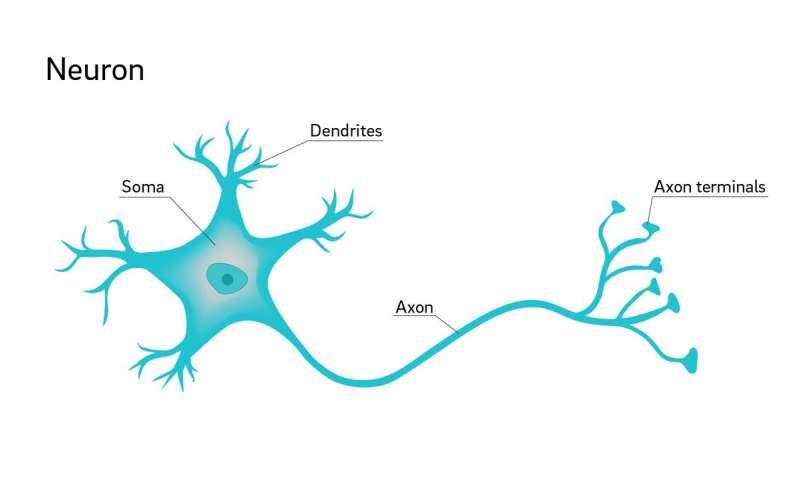
\includegraphics[width=\textwidth]{images/neural_networks/2-whyareneuron.jpg}
\end{figure}

\section{Architecture}

All CNN models has a similar architecture as it is shown in \ref{conv_full}. The input of such neural network is an image. CNN consists of a series of convolution and pooling operations followed by fully connected layers. These operations are described in the next paragraphs. 



\begin{figure}[h]
\caption{Convolutional neural network\cite{britz_2016}}
\label{conv_full}
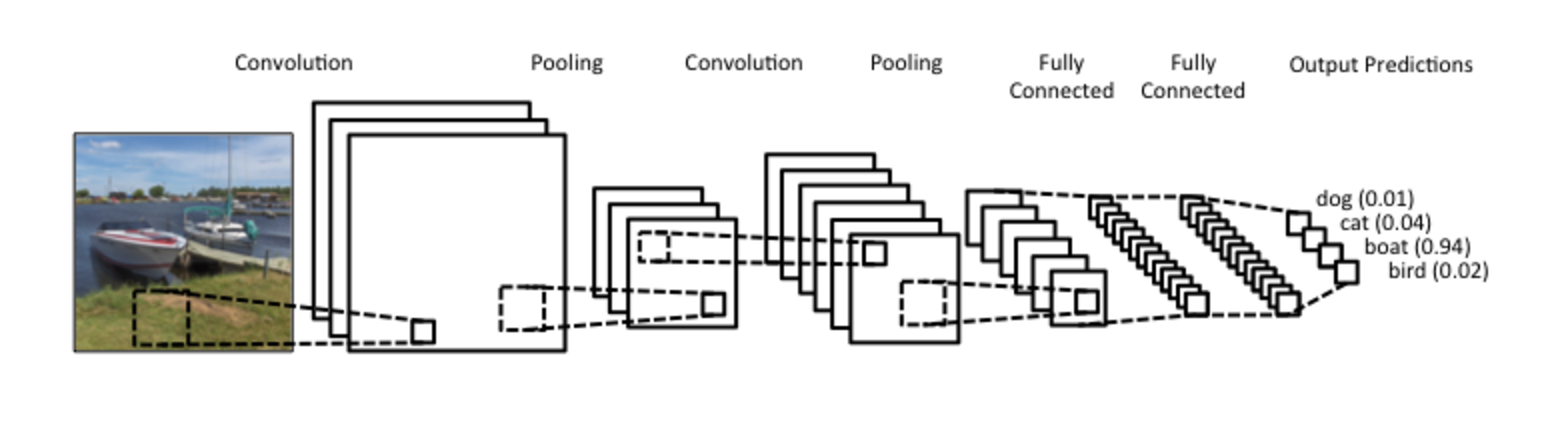
\includegraphics[width=\textwidth]{images/neural_networks/conv_full.png}
\end{figure}


\subsection{Convolutional layer} 

Convolutional layers consist of neurons placed in a grid of size $N \times M \times C$, where $N, M$ denotes width and height of convolutional filter and $C$ is number of channels in the previous layer (see \ref{convolutional_layer}). The filter moves from the left to the right with a certain stride until it completes processing width, then it moves down by the same stride to the beginning of the image    and repeats the process till the whole image is traversed. The process computes convolution as it is shown in \ref{conv_comp}. Calculated feature map is usually smaller than the input, but it is possible to preserve the same dimensionality by using padding to surround the input with zeros. 

\begin{figure}[h]
\caption{Convolutional layer\cite{cs231n}}
\label{convolutional_layer}
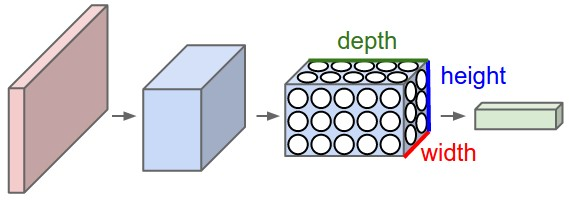
\includegraphics[width=\textwidth]{images/neural_networks/cnn.jpeg}
\end{figure}



\begin{figure}[h]
\caption{Convolution computation\cite{cs231n}}
\label{conv_comp}
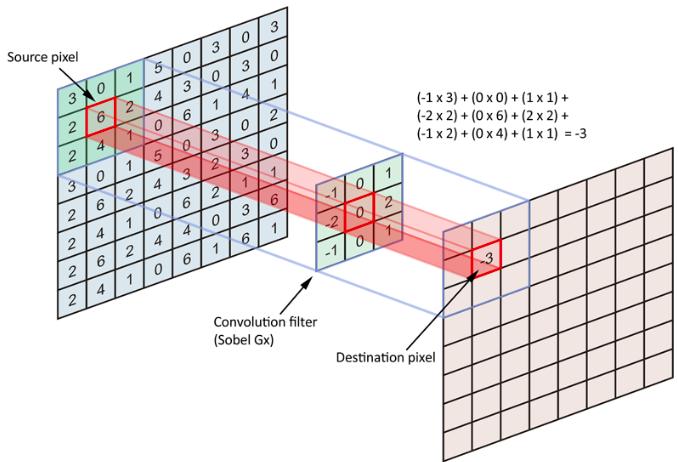
\includegraphics[width=\textwidth]{images/neural_networks/conv.png}
\end{figure}


\subsection{Non-linearity layer}

A non-linearity layer consists of an activation function that takes calculated feature map and creates the activation map as its output. The most common non-linearities used in CNN are sigmoid and ReLu \ref{non-linearity}.

\begin{figure}[h]
\subfloat[ReLu]{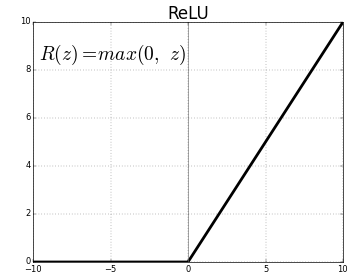
\includegraphics[width=0.6\textwidth]{images/neural_networks/relu.png}}\\
\subfloat[sigmoid]{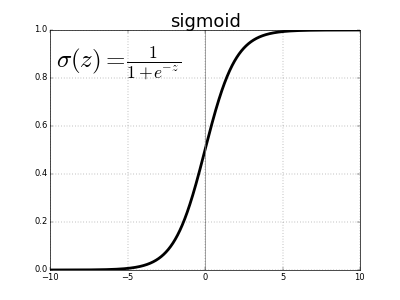
\includegraphics[width=0.68\textwidth]{images/neural_networks/sigmoid.png}}
\caption{Comparation of ReLu and sigmoid non-linearities}
\label{non-linearity}
\end{figure}
\subsection{Pooling layer}

After convolution, pooling layer is used to reduce the dimensionality which enables to reduce number of parameters. Two most common pooling operation are max and min pooling. It simply slides the input with particular stride and choose maximal or minimal value in predefined window (see \ref{pooling}). Pooling helps to not overfit CNN and can reduce the training time.


\begin{figure}[h]
\caption{Pooling layer\cite{cs231n}}
\label{pooling}
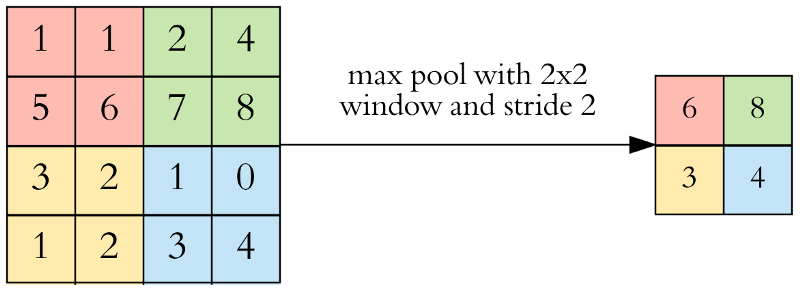
\includegraphics[width=\textwidth]{images/neural_networks/pooling.png}
\end{figure}

\subsection{Fully connected layer}

In fully connected layers, each neuron is connected to every neuron in the previous layer just like in feedforward neural networks.

\section{Training of CNN}

In this section, we will discuss how CNN are trained.

\subsection{Backpropagation}

For training CNN we should prepare training dataset as CNN belongs to supervised learning techniques. During training process, the network performs a forward pass for each example in training dataset. Computed output is compared to corresponding ground truth,  then loss is calculated and the error is backpropagated to change parameters of the network. The goal is to find such weights and biases for every neuron that the output is as close as possible to ground truth. That process is called backpropagation and was described in \cite{rumelhart_hinton_williams_1986}.

Each neural network can have its own loss function depending on what its output is. The most common loss function used for backpropagation is 

\begin{equation}
L = \frac{1}{2n}\sum_x\norm{y(x) - a(x)}^2	, 
\end{equation}

where $n$ denotes number of training inputs $x$, $y(x)$ label corresponding to the input $x$ and $a$ is network's output.

To update weight and biases we use gradient descent:

\begin{equation}
\omega = \omega - \eta \frac{\partial L}{\partial \omega}
\end{equation}
\begin{equation}
b = b - \eta \frac{\partial L}{\partial b}
\end{equation}

\subsection{Overfitting}

Overfitting is one of the biggest problem in machine learning. Overfitting means that a model performs well on a training dataset, but fails on test data. To solve this problem in neural networks, we can use so-called dropout. During each training step, individual neuron can be dropped out of the net with probability $1 - p$ or kept with probability $p$, so that only a reduced network is trained. The removed neurons are then reinserted into the network with unchanged weights. This methods not only decreases overfitting, but also improves training speed. 

\chapter{Used networks}
\section{ResNet}

Residual networks described in \cite{he_zhang_ren_sun_2016} are classification networks with image as the input and object class and confidence score as the output. In this paper they introduced shorcut connections that are widely used in modern neural networks.  One of the biggest problem with training deep neural networks is vanishing and exploding gradient. During backpropagation a lot of small or large numbers are multiplied to compute gradients. When the network is deep, multiplying of small numbers will become zero (vanished) and multiplying of large numbers will explode. Normally we expect deeper neural network will have more accurate predictions, but the opposite is true, and this degradation problem is caused by vanishing gradient.

This problem can be solved by adding shortcut connection which adds the input to the output after few weight layers, hence the output is $H(x) = F(x) + x$ (see \ref{resnet_block}). 

There are two types of residual connections. The identity shortcuts can be directly used when both input and output have the same dimension, or extra zero padding can be used when dimensions change. In both cases not extra parameters are needed. 

Comparing plain and residual network with 34 layers (see \ref{resnet}) Top-1 error drops from 28.54\% to 25.03\%. On the other hand, if we compare smaller network with 18 layers, Top-1 error changes from 27.94\% to 27.88\%, which means shortcut connections perform better in deeper networks. 

\begin{figure}[h]
\caption{Residual block}
\label{resnet_block}
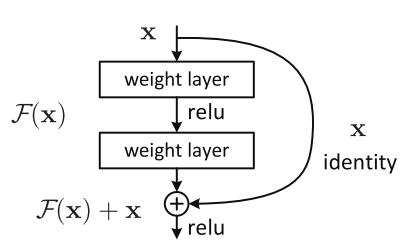
\includegraphics[width=.5\textwidth]{images/used_networks/resnet_block.png}
\end{figure}

\begin{figure}[h]
\caption{ResNet architecture}
\label{resnet}
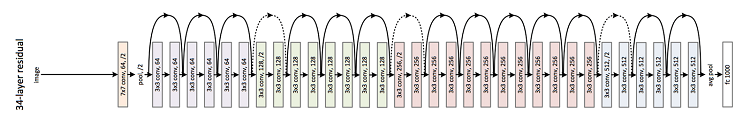
\includegraphics[width=\textwidth]{images/used_networks/resnet.png}
\end{figure}
\section{RetinaNet}
https://medium.com/@14prakash/the-intuition-behind-retinanet-eb636755607d

RetinaNet was proposed by Facebook AI Research and its features are described in \cite{lin_dollar_girshick_he_hariharan_belongie_2017} and \cite{lin_goyal_girshick_he_dollar_2017}. 

They proposed using anchor boxes instead of predicting bounding boxes. Sizes of the anchor boxes are predefined and used in further predictions. Thus, the network does not predict the final size of the object, but instead it only adjusts the size of the nearest anchor to the size of the object. 

Also they suggested a solution for object detection in different scales. Originally a pyramid of the same image at different scales was used to detect object. However, this solution is time consuming and has high memory demand. Instead a pyramid of features can be used. Although it is not such efficient for accurate object detection as image pyramids, it provides result faster and with less memory consumption. In \cite{lin_dollar_girshick_he_hariharan_belongie_2017} authors propose Feature Pyramid Network (FPN) which is fast like described pyramid of features, but more accurate. Its architecture is seen in \ref{fpn}.

The other solution, focal loss, solves class imbalance. Instead of normal cross entropy calculated by 

\begin{equation}
C(p, y) = -\sum_{i}y_i \ln p_i
\end{equation}  


scaled entropy is used using following equation:

\begin{equation}
C(p,y)=-\sum_i y_i(1-p_i)^{\lambda}\ln p_i.
\end{equation}

Here we can see focusing parameter $\lambda \geq 0$ which smoothly adjusts the rate at which easy examples are down weighted and thus training is focused on hard negatives. 



\begin{figure}[h]
\caption{Feature Pyramid Network}
\label{fpn}
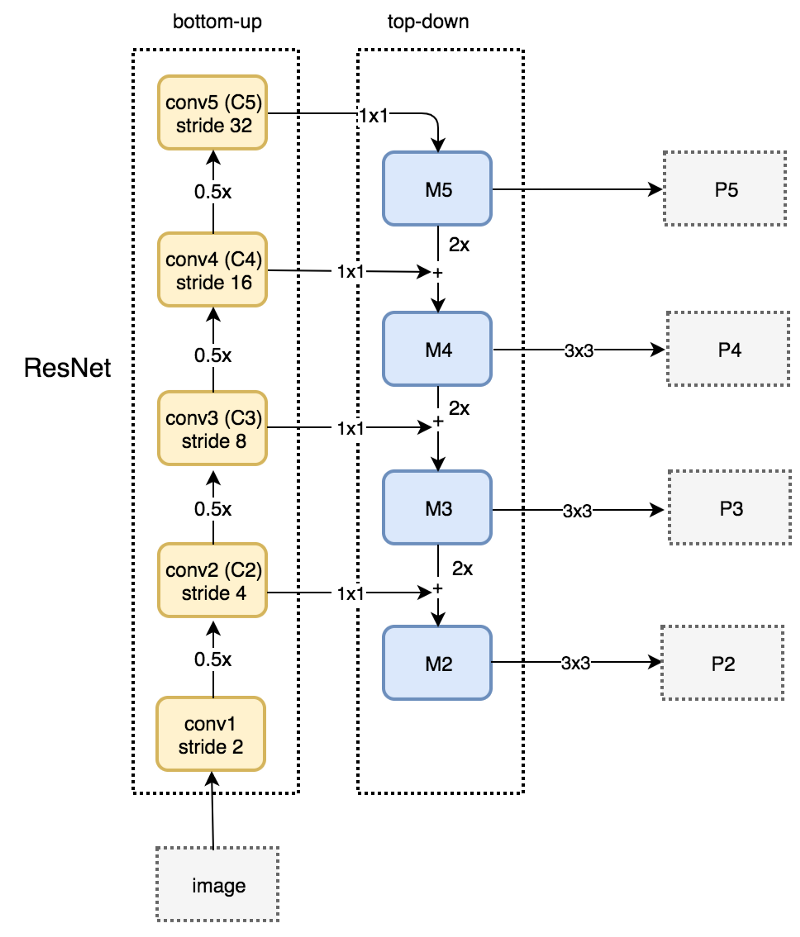
\includegraphics[width=\textwidth]{images/used_networks/fpn.png}
\end{figure}
\section{YOLO}

\subsection{YOLO v1}
A new approach for object detection, YOLO architecture, was presented in \cite{redmon_divvala_girshick_farhadi_2016}. A single neural network is used to predict both bounding boxes and class probabilities, hence an images is evaluated only once. Described system divides the input into a $S \times S$ grid and if the center of an object falls into a grid cell, this cell is responsible for detecting that object. Each cell also predicts $B$ bounding boxes and confidence score for them. Confidence is defined as 

\begin{equation}
score = Pr(Object)\cdot IoU^{truth}_{pred},
\end{equation}


where $Pr(Object)$ is probability of an object being inside that bounding box and $IoU^{truth}_{pred}$ denotes intersection over union between ground truth and prediction. 

Each bounding box consists of $\left(x, y, w, h, score\right)$, where $\left(x, y\right)$ represents the center of the box and $\left(w, h\right)$ denotes its width and height. Each grid cells also predicts conditional probability $C = Pr(Class_i|Object)$.

The model consists of 24 convolutional layers followed by 2 fully connected layers as it is shows in \ref{yolov1}.

\begin{figure}[h]
\caption{YOLO v1 architecture}
\label{yolov1}
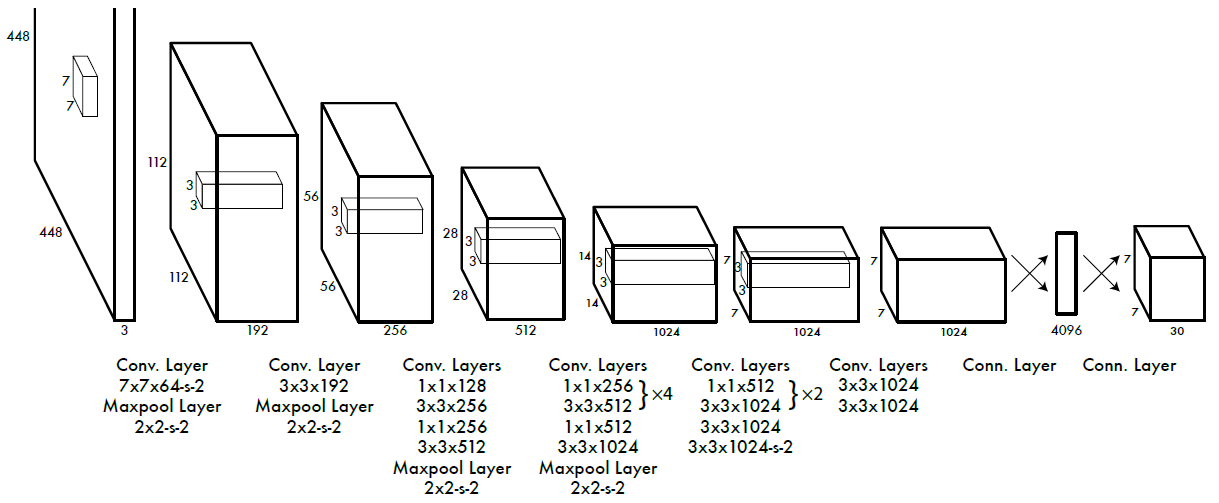
\includegraphics[width=\textwidth]{images/used_networks/yolov1.png}
\end{figure}

Training process optimizes loss function

\begin{multline}
\lambda_{coord}\sum_{i=0}^{S^2}\sum_{j=0}^{B}\textbf{1}_{ij}^{obj}\left[\left(x_i - \hat{x}_i\right)^2+\left(y_i + \hat{y}_i\right)^2\right]\\
+\lambda_{coord}\sum_{i=0}^{S^2}\sum_{j=0}^{B}\textbf{1}_{ij}^{obj}\left[\left(\sqrt{w_i} - \sqrt{\hat{w_i}}\right)^2+\left(\sqrt{h_i} + \sqrt{\hat{h}_i}\right)^2\right]\\
+\sum_{i=0}^{S^2}\sum_{j=0}^{B}\textbf{1}_{ij}^{obj}\left(C_i-\hat{C}_i\right)^2\\
+\lambda_{noobj}\sum_{i=0}^{S^2}\sum_{j=0}^{B}\textbf{1}_{ij}^{noobj}\left(C_i-\hat{C}_i\right)^2\\
+\sum_{i=0}^{S^2}\textbf{1}_{ij}^{obj}\sum_{c\in classes}\left(p_i(c) - \hat{p}_i(c)\right)^2
\end{multline},

where 
\begin{equation}
  \textbf{1}_{ij}^{obj}=\begin{cases}
    1, & \text{if there is an object}.\\
    0, & \text{otherwise},
  \end{cases}
\end{equation}
$\textbf{1}_{ij}^{noobj}$ is inverse function to $\textbf{1}_{ij}^{obj}$, $\lambda_{coord}$ and $\lambda_{noobj}$ are constant to increase the loss from bounding box coordinate prediction and decrease the loss from confidence prediction for boxes that does not contain objects. 

While YOLO v1 was faster than most of existing approaches for object detection, it had relatively low 57.9\% mAP on the VOC 2012 test set comparing to existing state of art. 

\subsection{YOLO v2}

New version of YOLO was introduced in \cite{redmon_farhadi_2017}. Authors of this state of art detector refers to it as a better, faster and stronger version of YOLO. For a better performance they added batch normalization and used images with bigger resolution to train the network. They also removed fully connected layers and used anchor boxes to predict bounding boxes, which lead to a small decrease in mAP from 69.5\% to 69.2\%, but it also increased a recall from 81\% to 88\%. We can see how applied changes improved network performance in \ref{yolov2_improve}.

\begin{figure}[h]
\caption{YOLO v2 improvement}
\label{yolov2_improve}
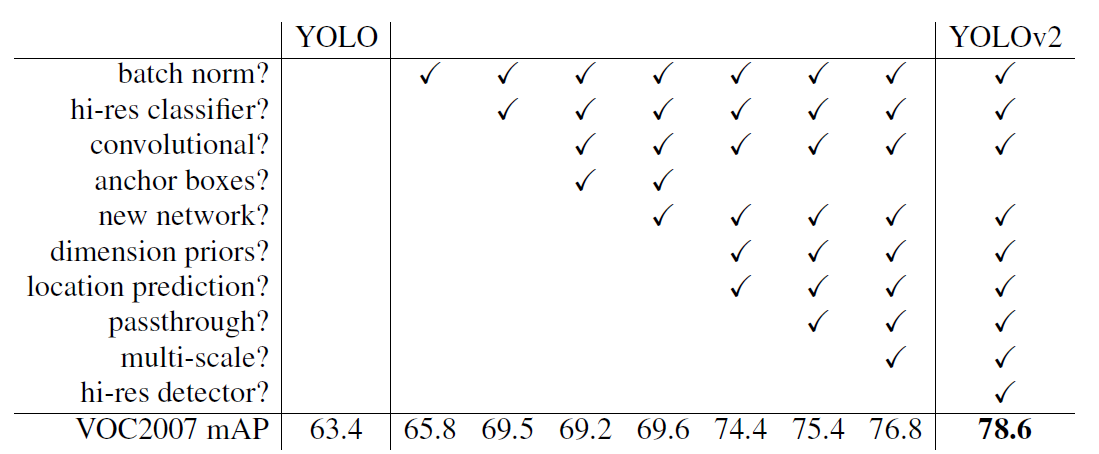
\includegraphics[width=\textwidth]{images/used_networks/yolov2_improve.png}
\end{figure}

They also proposed new classification network called Darknet-19\ref{darknet-19} to make YOLO even faster. We can see that Darknet-19 has many $1\times 1$ convolutions  to reduce the number of parameters. 

\begin{figure}[h]
\caption{Darknet-19}
\label{darknet-19}
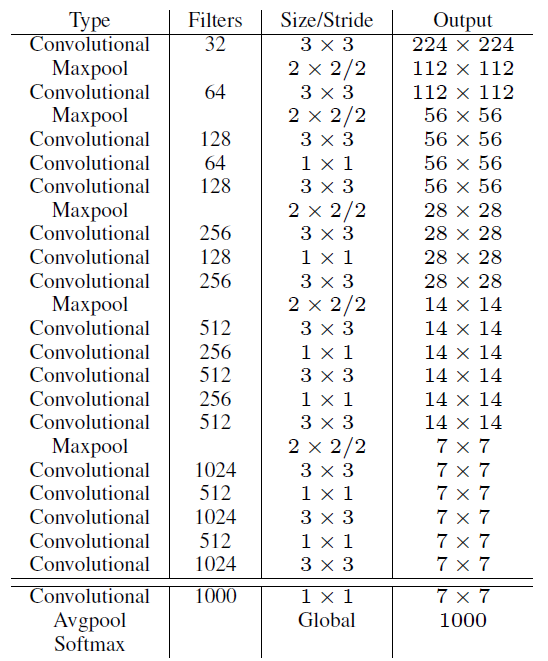
\includegraphics[width=\textwidth]{images/used_networks/yolov2_darknet.png}
\end{figure}

\subsection{YOLO v3}

The newest version of YOLO was presented in \cite{Redmon2018YOLOv3AI}. Similar to YOLOv2 it predicts bounding boxes using dimension clusters as anchor boxes. The network predicts 4 coordinates for each bounding box and for training they use sum of squared error loss. Objectness score for each bounding box is predicted using logistic regression, which should be 1 if the bounding box prior overlaps a ground truth object by more than any other bounding box prior. 

They also use 3 different scales for prediction, which is similar to feature pyramid networks. Features are now extracted with deeper  extractor called Darknet-53 (see \ref{darknet-53}) with shortcut connections.

\begin{figure}[h]
\caption{Darknet-53}
\label{darknet-53}
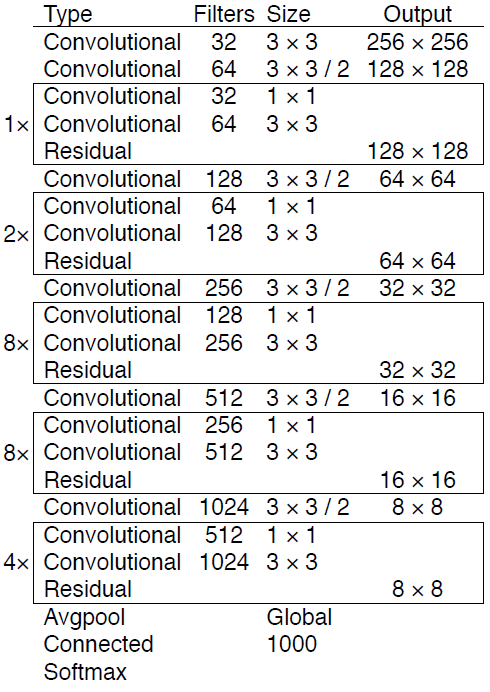
\includegraphics[width=\textwidth]{images/used_networks/yolov3_darknet.png}
\end{figure}

Comparing to other state of art solutions, YOLO v3 has similar performance, but it is much faster as it is seen in \ref{yolov3-compare}

\begin{figure}[h]
\caption{YOLO v3 comparation}
\label{yolov3-compare}
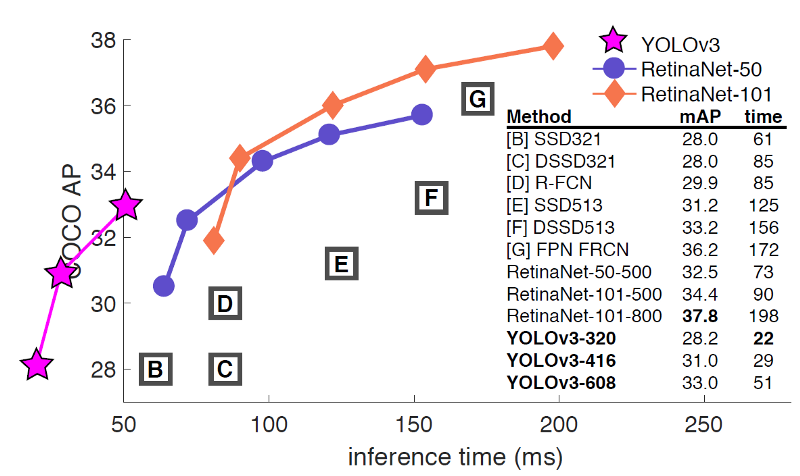
\includegraphics[width=\textwidth]{images/used_networks/yolov3_comparasion.png}
\end{figure}
\section{SqueezeDet}

SqueezeDet (https://arxiv.org/pdf/1612.01051.pdf) is a single stage detection pipeline inspired by YOLO. The main difference between two architectures is that SqueezeDet uses SqueezeNet (https://arxiv.org/pdf/1602.07360.pdf) for feature extraction.

The building brick of SqueezeNet is called fire module \ref{fire_squeezenet}. Each fire module contains a squeeze layer and an expand layer. Squeeze layers replace 3$\times$3 filters by 1$\times$1 filters to reduce computation complexity 9 times. Following expand layers contain number of 1$\times$1  and 3$\times$3 kernels.	Squeeze layers reduce depth of calculated feature map, which means the following 3$\times$3 filters in expand layers have to do fewer computation. Thanks to its architecture, SqueezeDet can be faster and smaller comparing to other state-of-art solutions (see \ref{squeezedet_comparasion}), and so can be efficiently used on embedded system. 

\begin{figure}[h]
\caption{Fire module in SqueezeNet}
\label{fire_squeezenet}
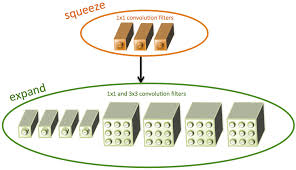
\includegraphics[width=.5\textwidth]{images/used_networks/fire_squeezenet.jpeg}
\end{figure}

\begin{figure}[h]
\caption{SqueezeDet comparison with other state-of-art solutions}
\label{squeezedet_comparasion}
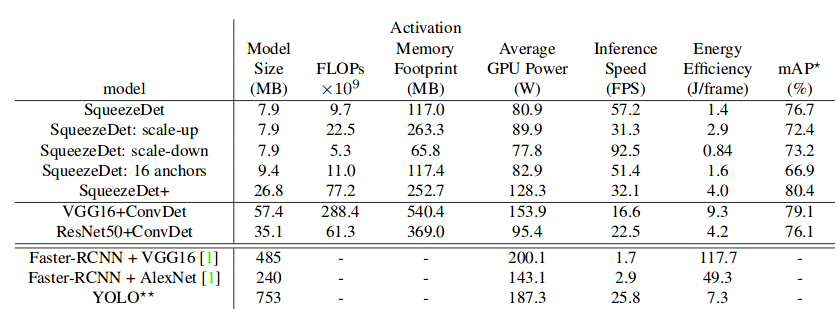
\includegraphics[width=\textwidth]{images/used_networks/squeezedet_comparation.png}
\end{figure}

\chapter{Experiments}

As soon as ResNet is just a classification network without bounding boxes proposal, we decided to evaluate performance of networks for both detection and classification, hence, RetinaNet, YOLOv3.
\section{Inference time evaluation}

For computing on the edge, we should ensure as small as possible time delay between receiving input data, in this case stream frame,  and providing output data to a user. Time of object detection and classification can be the biggest bottleneck in such systems, therefore it is necessary to choose such architecture that provides the best result with the least possible inference time. We compared necessary time to process one image frame on Jetson AGX Xavier with other 2 different machines, their CPU and GPU specifications are mentioned in tables \ref{malaria-tech-spec} and \ref{my-tech-spec}. Videos for this evaluation were taken from video databases with free access, like YouTube or Pexels. All videos have different camera view with various object count, video resolution and FPS, which can affect neural network detector performance. Video samples are presented on \ref{fig:samples}, where obvious difference between videos can be noticed.  As it is shown in tables \ref{yolo-evaluation} and \ref{retina-eval}, PC1 performs best for both YOLO and RetinaNet, while PC2 has the worst performance. Jetson AVX Xavier has 2.5 times worse performance with YOLO and 4 times worse with RetinaNet comparing to PC1. The difference in performance of YOLO and RetinaNet on Jetson AVX Xavier is caused by frameworks used for computation. Darknet used with YOLO is optimized for utilizing of Tensor Cores in Jetson, while TensorFlow is not able to use Tensor Cores for faster matrix calculation. This problem can be solved by accelerating inference in TensorFlow with TensorRT. Unfortunately, in case of RetinaNet there are layers like $Exit$, $Switch$, $LoopCond$, $LogicalAnd$, $Enter$ etc. in graph that are not fully supported in TensorRT, which means TensorRT optimizes only known layers and the resulting network does not gain any speed improvement. The possible solution for this problem could be writing custom layer converter for a network graph.


\begin{table}[htb]
	\centering
	\resizebox{.7\textwidth}{!}{%
		\begin{tabular}{|c|c|}
			\hline
			CPU     & Intel(R) Core(TM) i7-8700K CPU @ 3.70GHz       \\ \hline
			GPU     & 3584-core 11Gb GeForce GTX 1080 Ti @ 1582MHz \\ \hline
		\end{tabular}%
	}
	\caption{PC1 technical specification}
	\label{malaria-tech-spec}
\end{table}

\begin{table}[htb]
	\centering
	\resizebox{.7\textwidth}{!}{%
		\begin{tabular}{|c|c|}
			\hline
			CPU     & Intel(R) Core(TM) i5-7300HQ CPU @ 2.50GHz       \\ \hline
			GPU     & 640-core 4Gb GeForce GTX 1050 @ 1404MHz \\ \hline
		\end{tabular}%
	}
	\caption{PC2 technical specification}
	\label{my-tech-spec}
\end{table}
% Please add the following required packages to your document preamble:
% \usepackage{multirow}
% \usepackage[table,xcdraw]{xcolor}
% If you use beamer only pass "xcolor=table" option, i.e. \documentclass[xcolor=table]{beamer}
\begin{table}[]
\resizebox{\textwidth}{!}{
\begin{tabular}{|c|c|c|}
\hline
\cellcolor[HTML]{C0C0C0}                                                              & \cellcolor[HTML]{C0C0C0}{\color[HTML]{333333} }                               & \cellcolor[HTML]{C0C0C0}                                            \\
\cellcolor[HTML]{C0C0C0}                                                              & \cellcolor[HTML]{C0C0C0}{\color[HTML]{333333} }                               & \cellcolor[HTML]{C0C0C0}                                            \\
\multirow{-3}{*}{\cellcolor[HTML]{C0C0C0}\textbf{Video file}}                         & \multirow{-3}{*}{\cellcolor[HTML]{C0C0C0}{\color[HTML]{333333} \textbf{FPS}}} & \multirow{-3}{*}{\cellcolor[HTML]{C0C0C0}\textbf{Video Resolution}} \\ \hline
5.4 4K Camera Road in Thailand.mp4                                                    & 30                                                                            & 1280x720                                                            \\ \hline
Cars Driving On Street.mp4                                                            & 30                                                                            & 1920x1080                                                           \\ \hline
Cars On Highway.mp4                                                                   & 25                                                                            & 1920x1080                                                           \\ \hline
Cars On The Road.mp4                                                                  & 50                                                                            & 1280x720                                                            \\ \hline
City Traffic.mp4                                                                      & 30                                                                            & 1920x1088                                                           \\ \hline
Day Traffic Sample Video Dataset.mp4                                                  & 30                                                                            & 432x240                                                             \\ \hline
Pedestrian and Traffic, Human Activity Recognition Video ,DataSet By UET Peshawar.mp4 & 30                                                                            & 1280x720                                                            \\ \hline
Pexels Videos 1601538.mp4                                                             & 25                                                                            & 1920x1080                                                           \\ \hline
Pexels Videos 2577.mp4                                                                & 30                                                                            & 1920x1088                                                           \\ \hline
Pexels Videos 2670.mp4                                                                & 25                                                                            & 1920x1088                                                           \\ \hline
Pexels Videos 3047.mp4                                                                & 30                                                                            & 1920x1088                                                           \\ \hline
Pexels Videos 948404.mp4                                                              & 24                                                                            & 3840x2178                                                           \\ \hline
moderate\_traffic.mp4                                                                 & 30                                                                            & 1280x720                                                            \\ \hline
\end{tabular}
}
\caption{Characteristics of video for inference time evaluation}
	\label{video_characteristics}
\end{table}

% Please add the following required packages to your document preamble:												
% \usepackage{multirow}												
% \usepackage[table,xcdraw]{xcolor}												
% If you use beamer only pass "xcolor=table" option, i.e. \documentclass[xcolor=table]{beamer}												
\begin{table}[]		

 \catcode`\-=12										
\begin{tabular}{|c|c|c|}												
\hline												
\cellcolor[HTML]{C0C0C0}{\color[HTML]{333333} }                                 & \cellcolor[HTML]{C0C0C0}{\color[HTML]{333333} }                                   & \cellcolor[HTML]{C0C0C0}{\color[HTML]{333333} }                                                   \\												
\cellcolor[HTML]{C0C0C0}{\color[HTML]{333333} }                                 & \cellcolor[HTML]{C0C0C0}{\color[HTML]{333333} }                                   & \cellcolor[HTML]{C0C0C0}{\color[HTML]{333333} }                                                   \\												
\multirow{-3}{*}{\cellcolor[HTML]{C0C0C0}{\color[HTML]{333333} \textbf{Model}}} & \multirow{-3}{*}{\cellcolor[HTML]{C0C0C0}{\color[HTML]{333333} \textbf{Machine}}} & \multirow{-3}{*}{\cellcolor[HTML]{C0C0C0}{\color[HTML]{333333} \textbf{Inference time {[}ms{]}}}} \\ \hline												
& Jetson Xavier                                                                     & 123                                                                                               \\ \cline{2-3}												
& PC1                                                                               & 35                                                                                                \\ \cline{2-3}												
\multirow{-3}{*}{YOLOv3 416x416}                                                & PC2                                                                               & 175                                                                                               \\ \hline												
& Jetson Xavier                                                                     & 139                                                                                               \\ \cline{2-3}												
& PC1                                                                               & 39                                                                                                \\ \cline{2-3}												
\multirow{-3}{*}{YOLOv3 608x608}                                                & PC2                                                                               & 208                                                                                               \\ \hline												
& Jetson Xavier                                                                     & 200                                                                                               \\ \cline{2-3}												
& PC1                                                                               & 52                                                                                                \\ \cline{2-3}												
\multirow{-3}{*}{RetinaNet}                                                     & PC2                                                                               & 228                                                                                               \\ \hline												
& Jetson Xavier                                                                     & 25                                                                                                \\ \cline{2-3}												
& PC1                                                                               & 8                                                                                                 \\ \cline{2-3}												
\multirow{-3}{*}{squeezeDet}                                                    & PC2                                                                               & 24                                                                                                \\ \hline												
\end{tabular}	
\caption{Inference time evaluation}
\label{inference_time}										
\end{table}												


\begin{figure}[]
	\centering
	\subfloat[5.4 4K Camera Road in Thailand.mp4]{
		\centering
		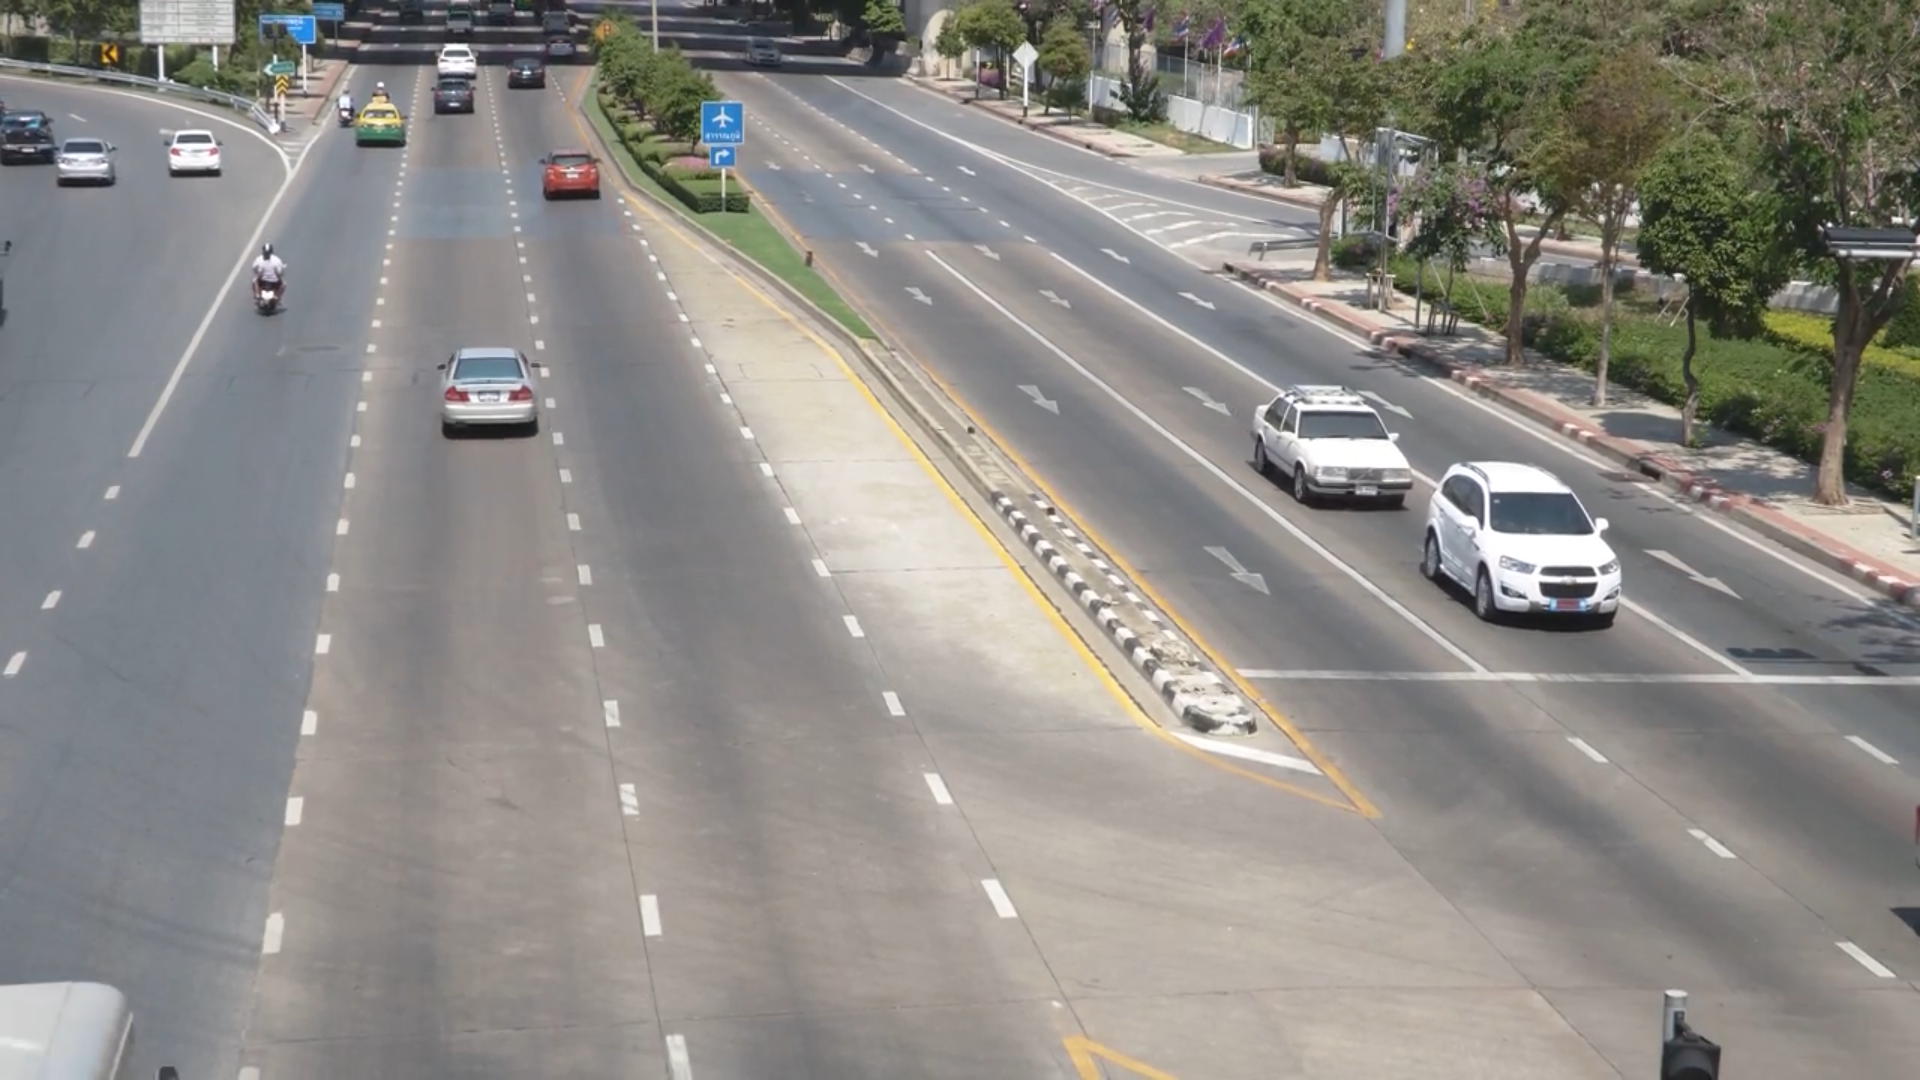
\includegraphics[width=.5\linewidth]{images/experiments/5_4.png}\label{fig:image1}
	}
	\subfloat[Cars Driving On Street.mp4]{
		\centering
		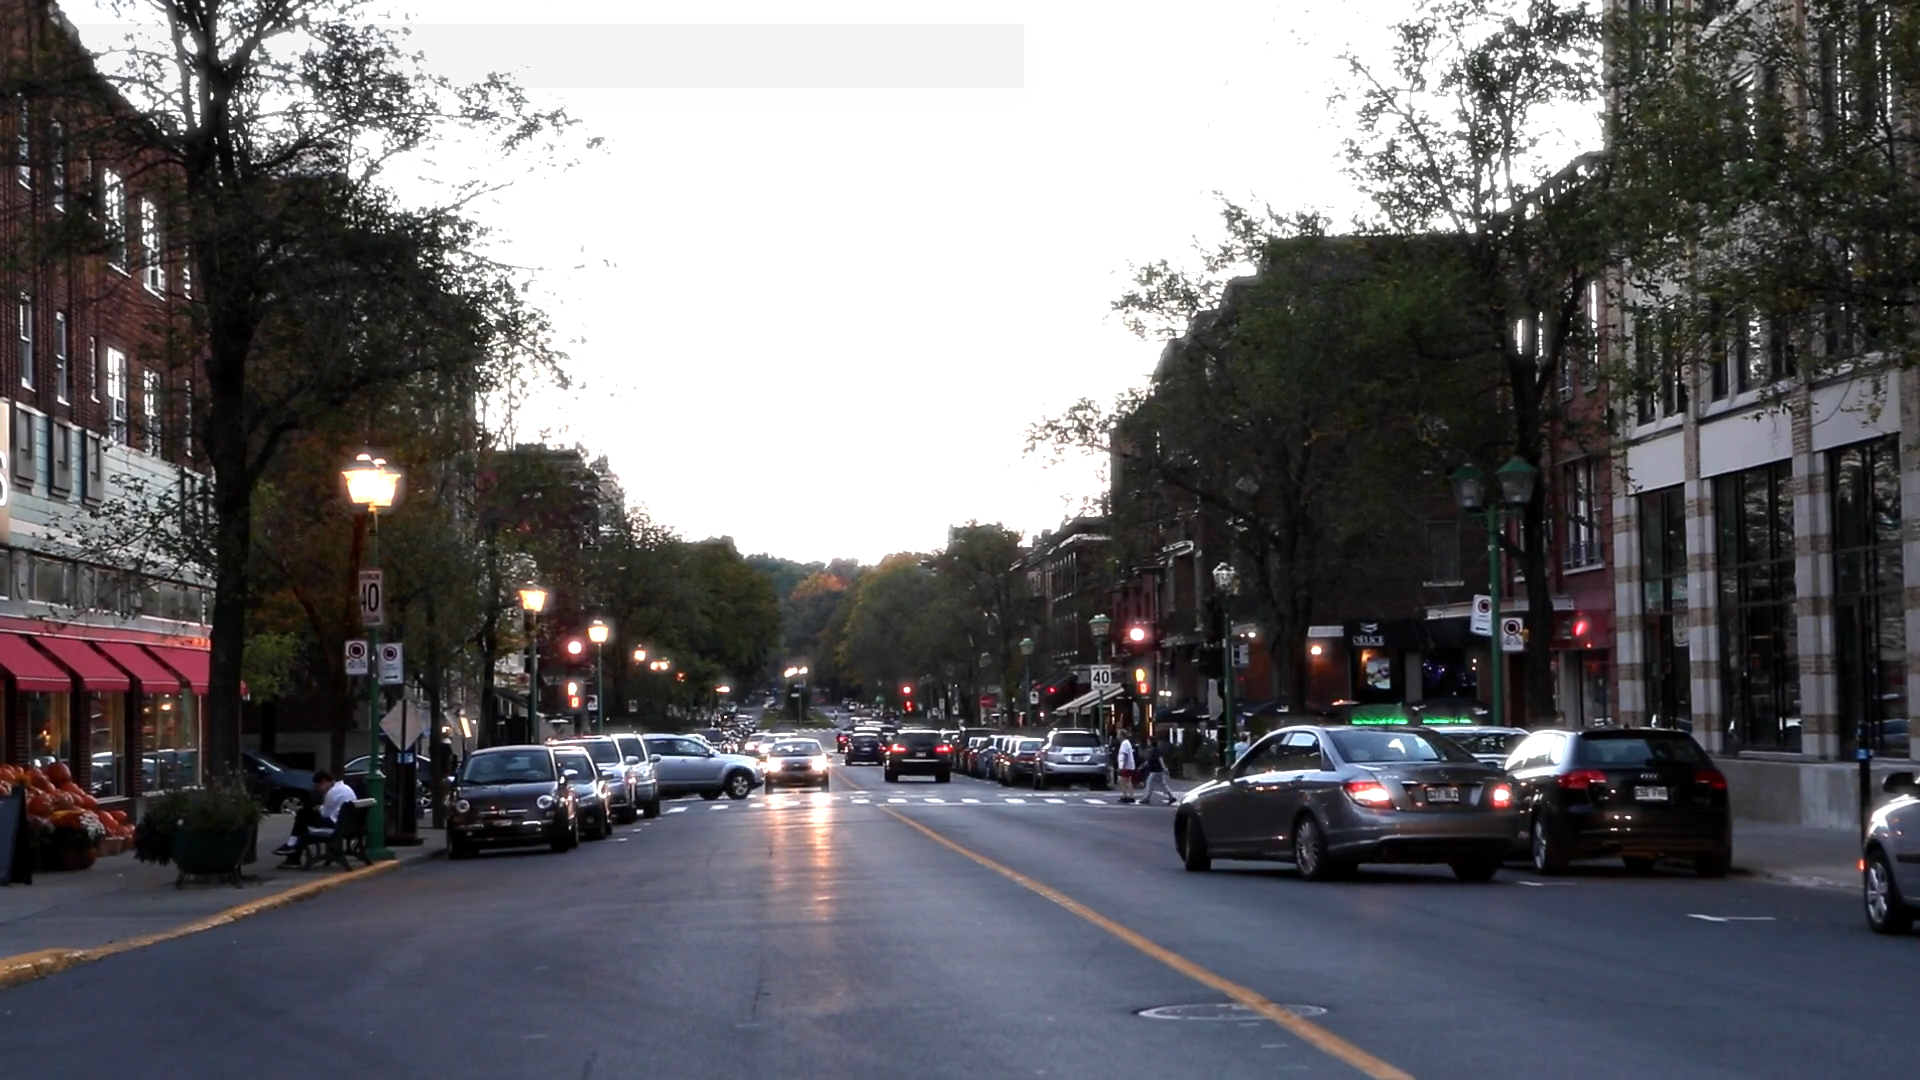
\includegraphics[width=.5\linewidth]{images/experiments/cars_on_streets.png}\label{fig:image1}
	}
	\hfill
		
	\bigskip
	\subfloat[Cars On Highway.mp4]{
		\centering
		
		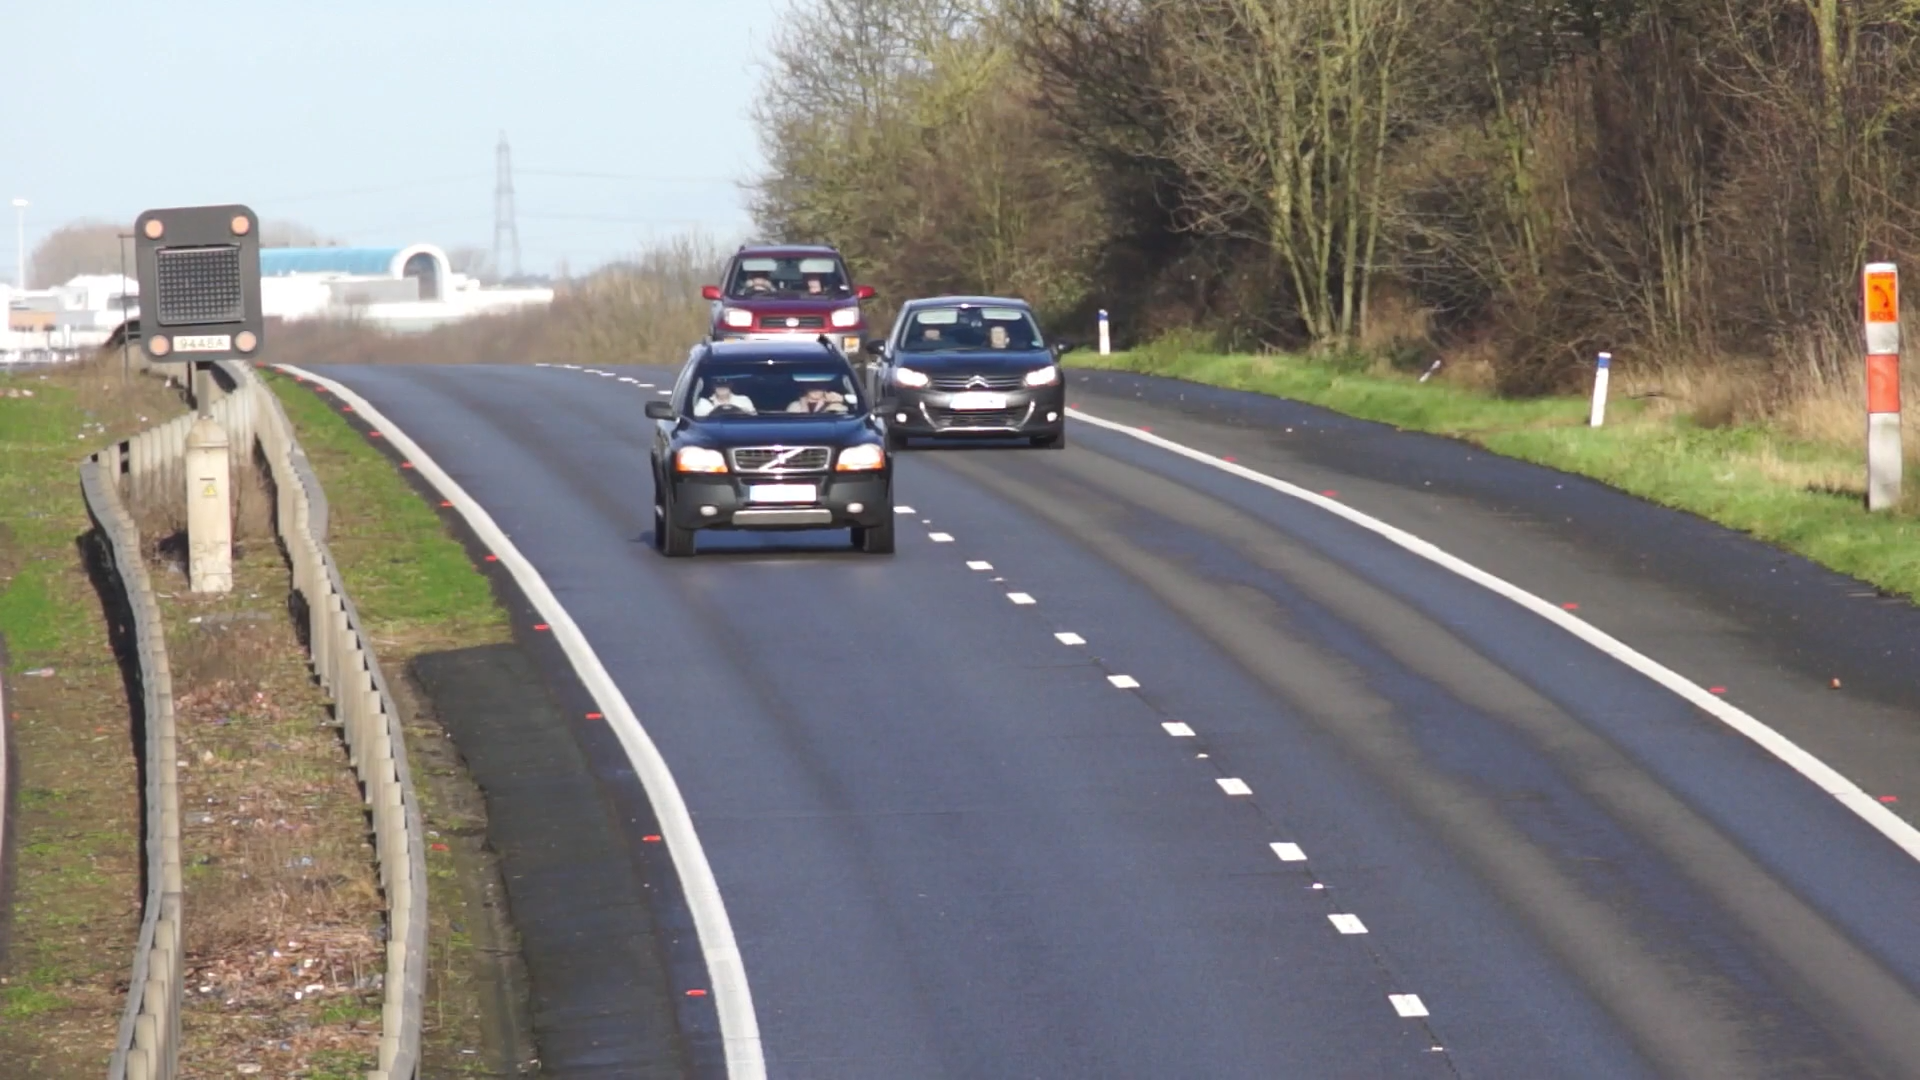
\includegraphics[width=.5\linewidth]{images/experiments/cars_highway.png}
		\label{fig:cars_highway}
	}
	\subfloat[Cars On The Road.mp4]{
		\centering
		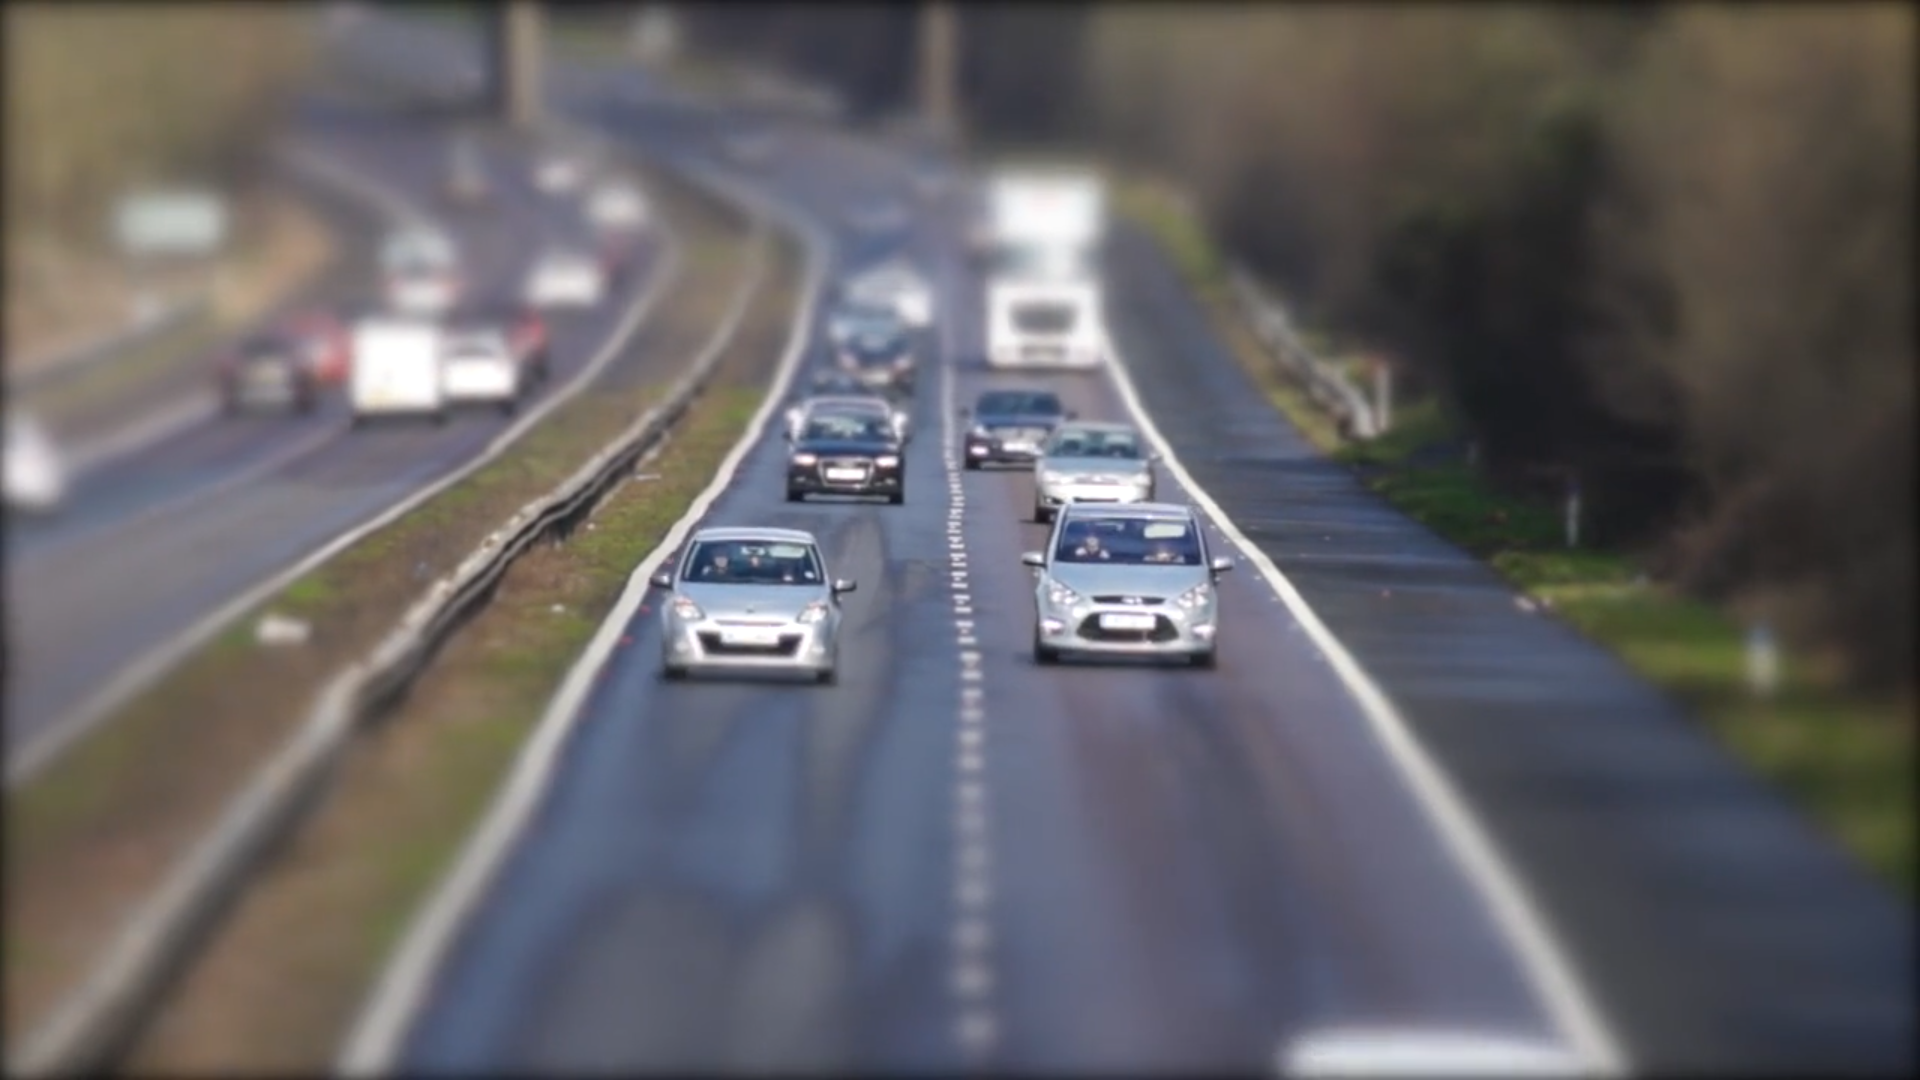
\includegraphics[width=.5\linewidth]{images/experiments/cars_road.png}\label{fig:image1}
	}
	\hfill
	\bigskip
	\subfloat[City Traffic.mp4]{
		\centering
		
		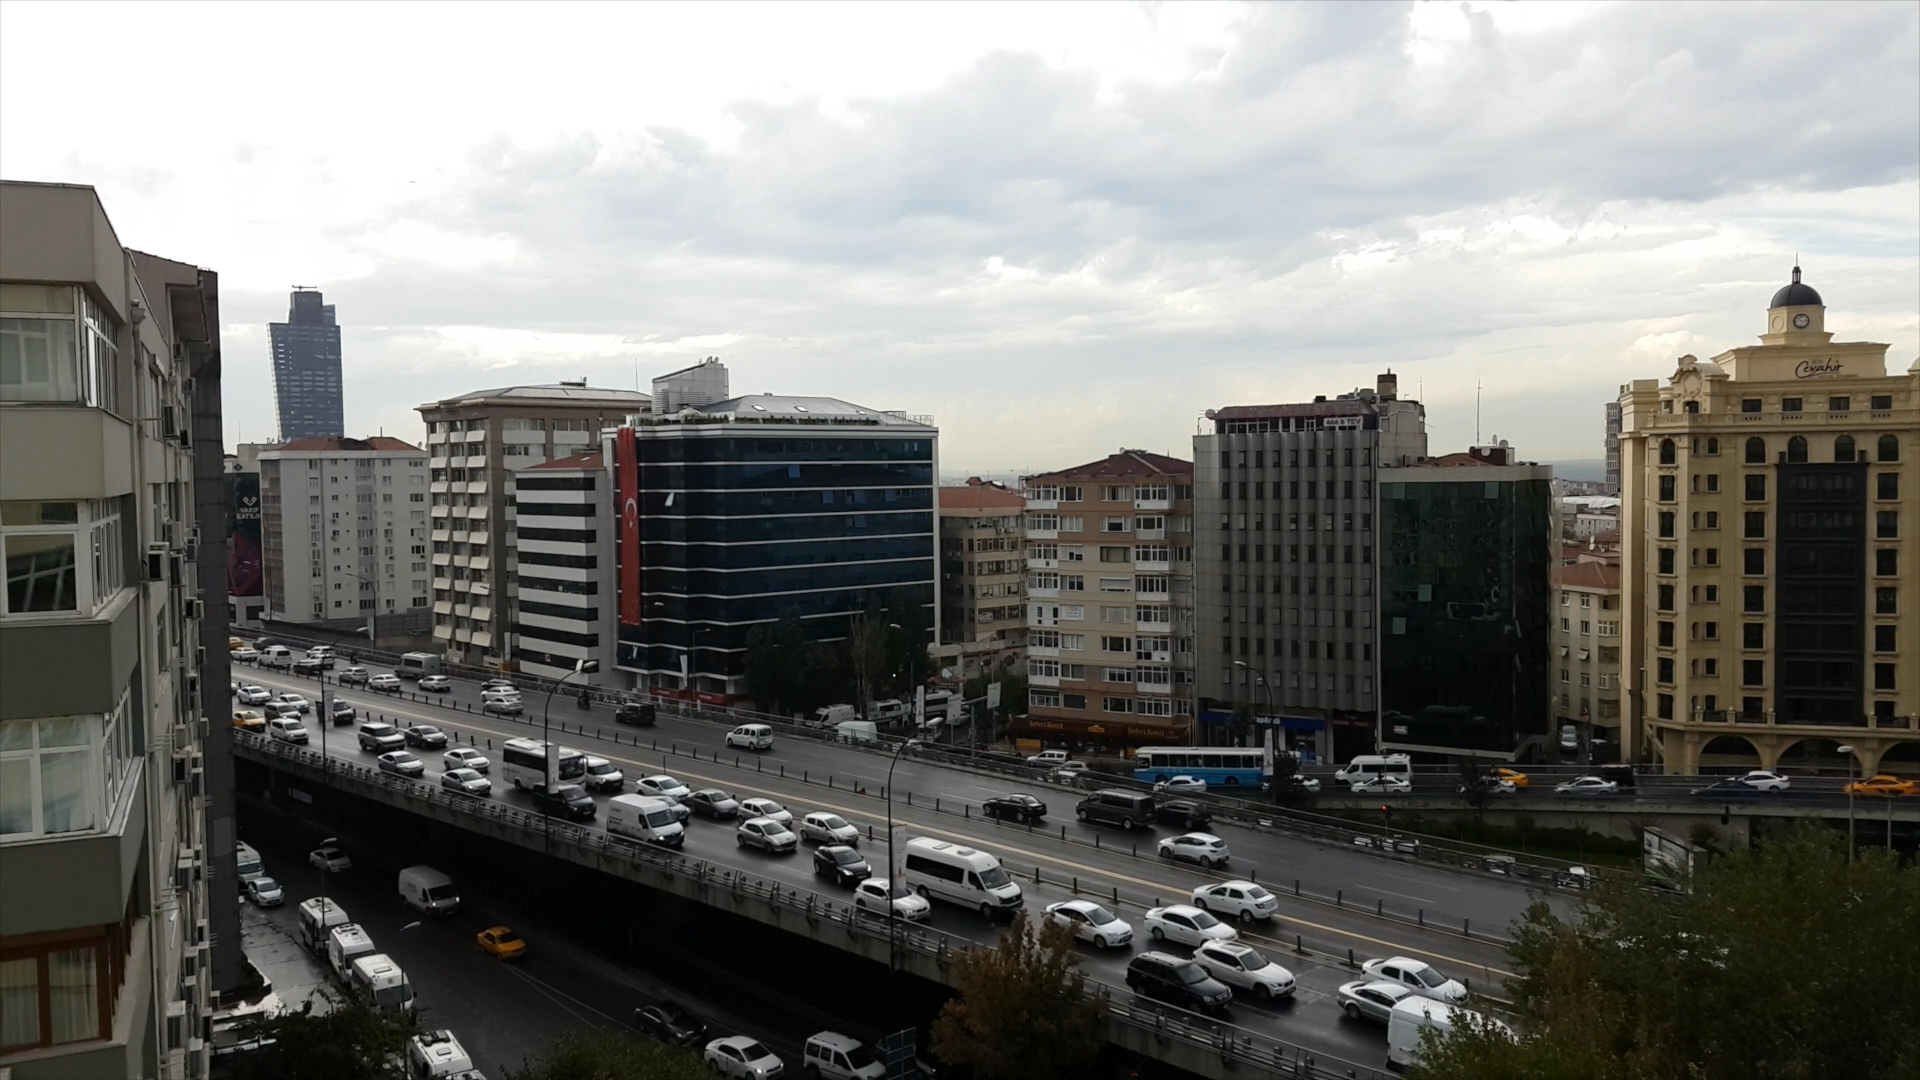
\includegraphics[width=.5\linewidth]{images/experiments/city_traffic.png}\label{fig:image1}
	}
	\subfloat[Day Traffic Sample Video Dataset.mp4]{
		\centering
		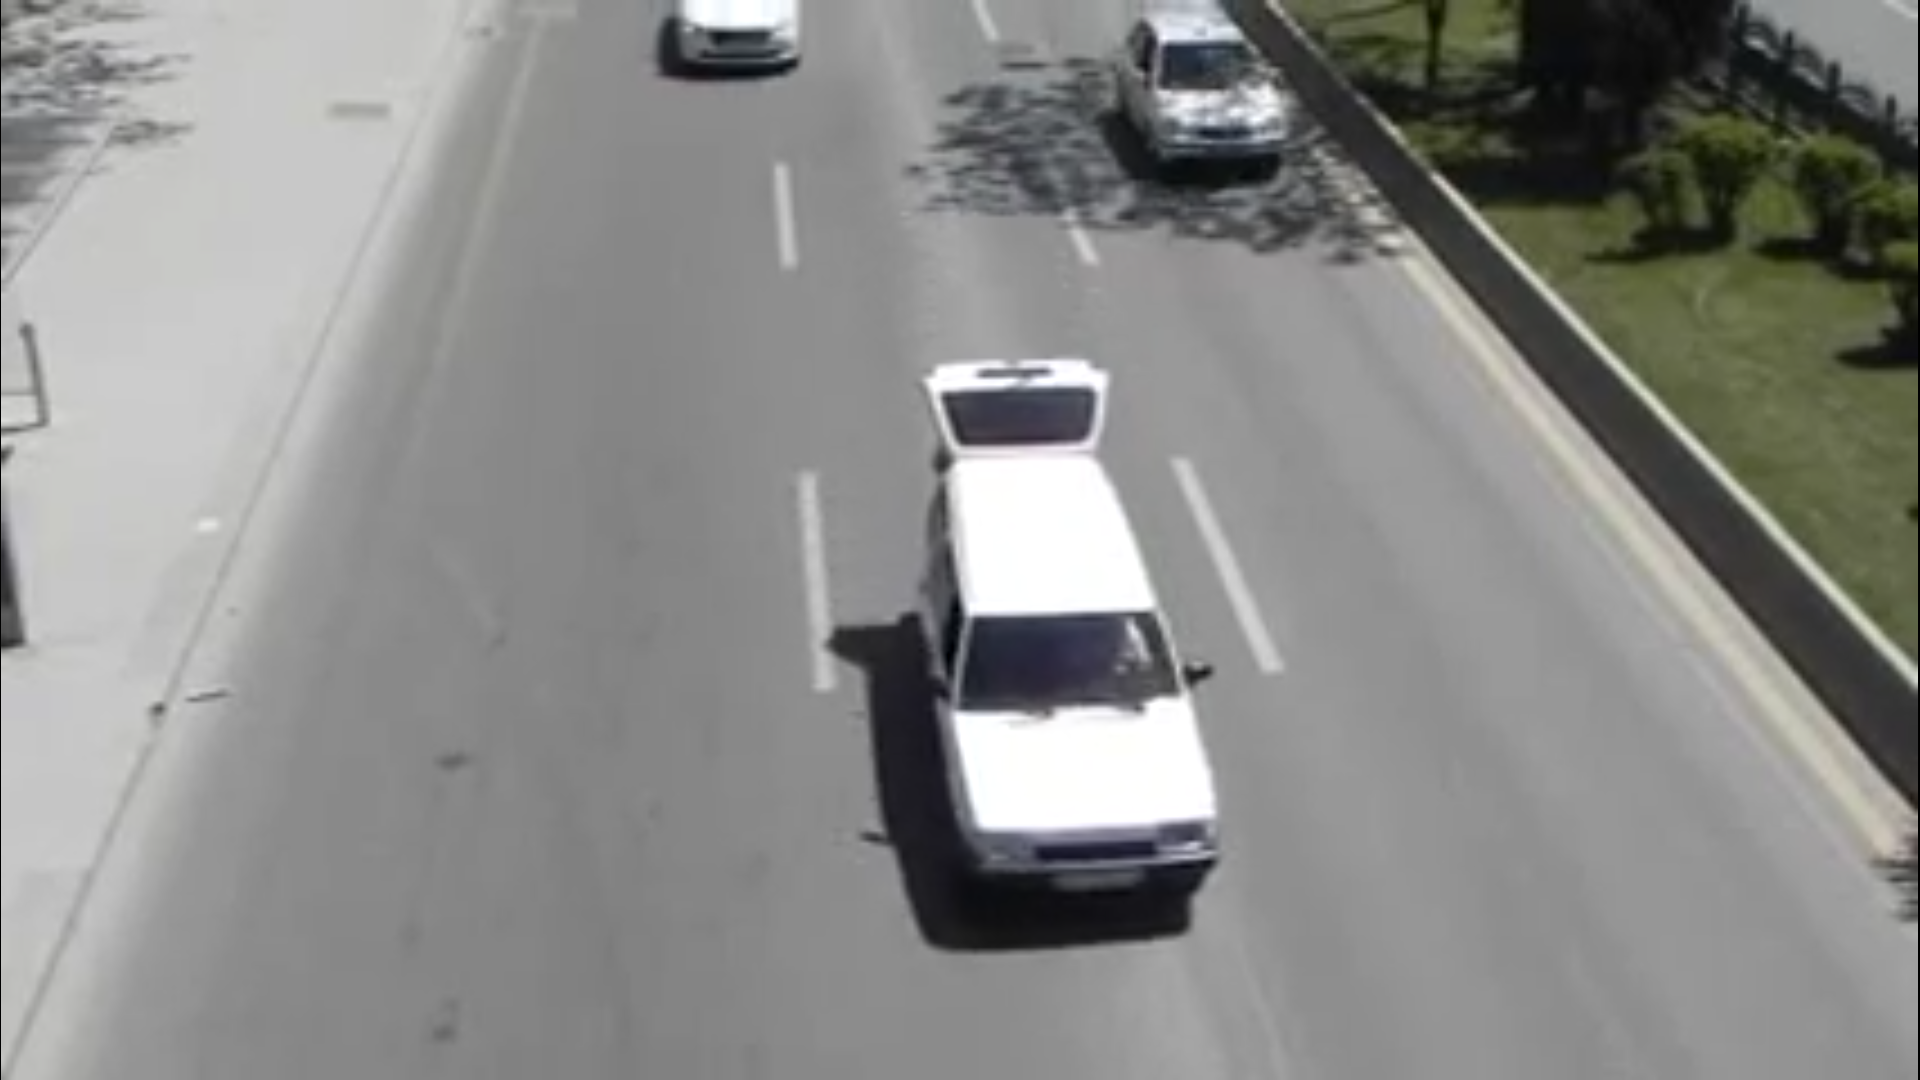
\includegraphics[width=.5\linewidth]{images/experiments/day_traffic.png}\label{fig:image1}
	}
	\hfill
	\bigskip
	\subfloat[Pedestrian and Traffic, Human Activity Recognition Video ,DataSet By UET Peshawar.mp4]{
		\centering
		
		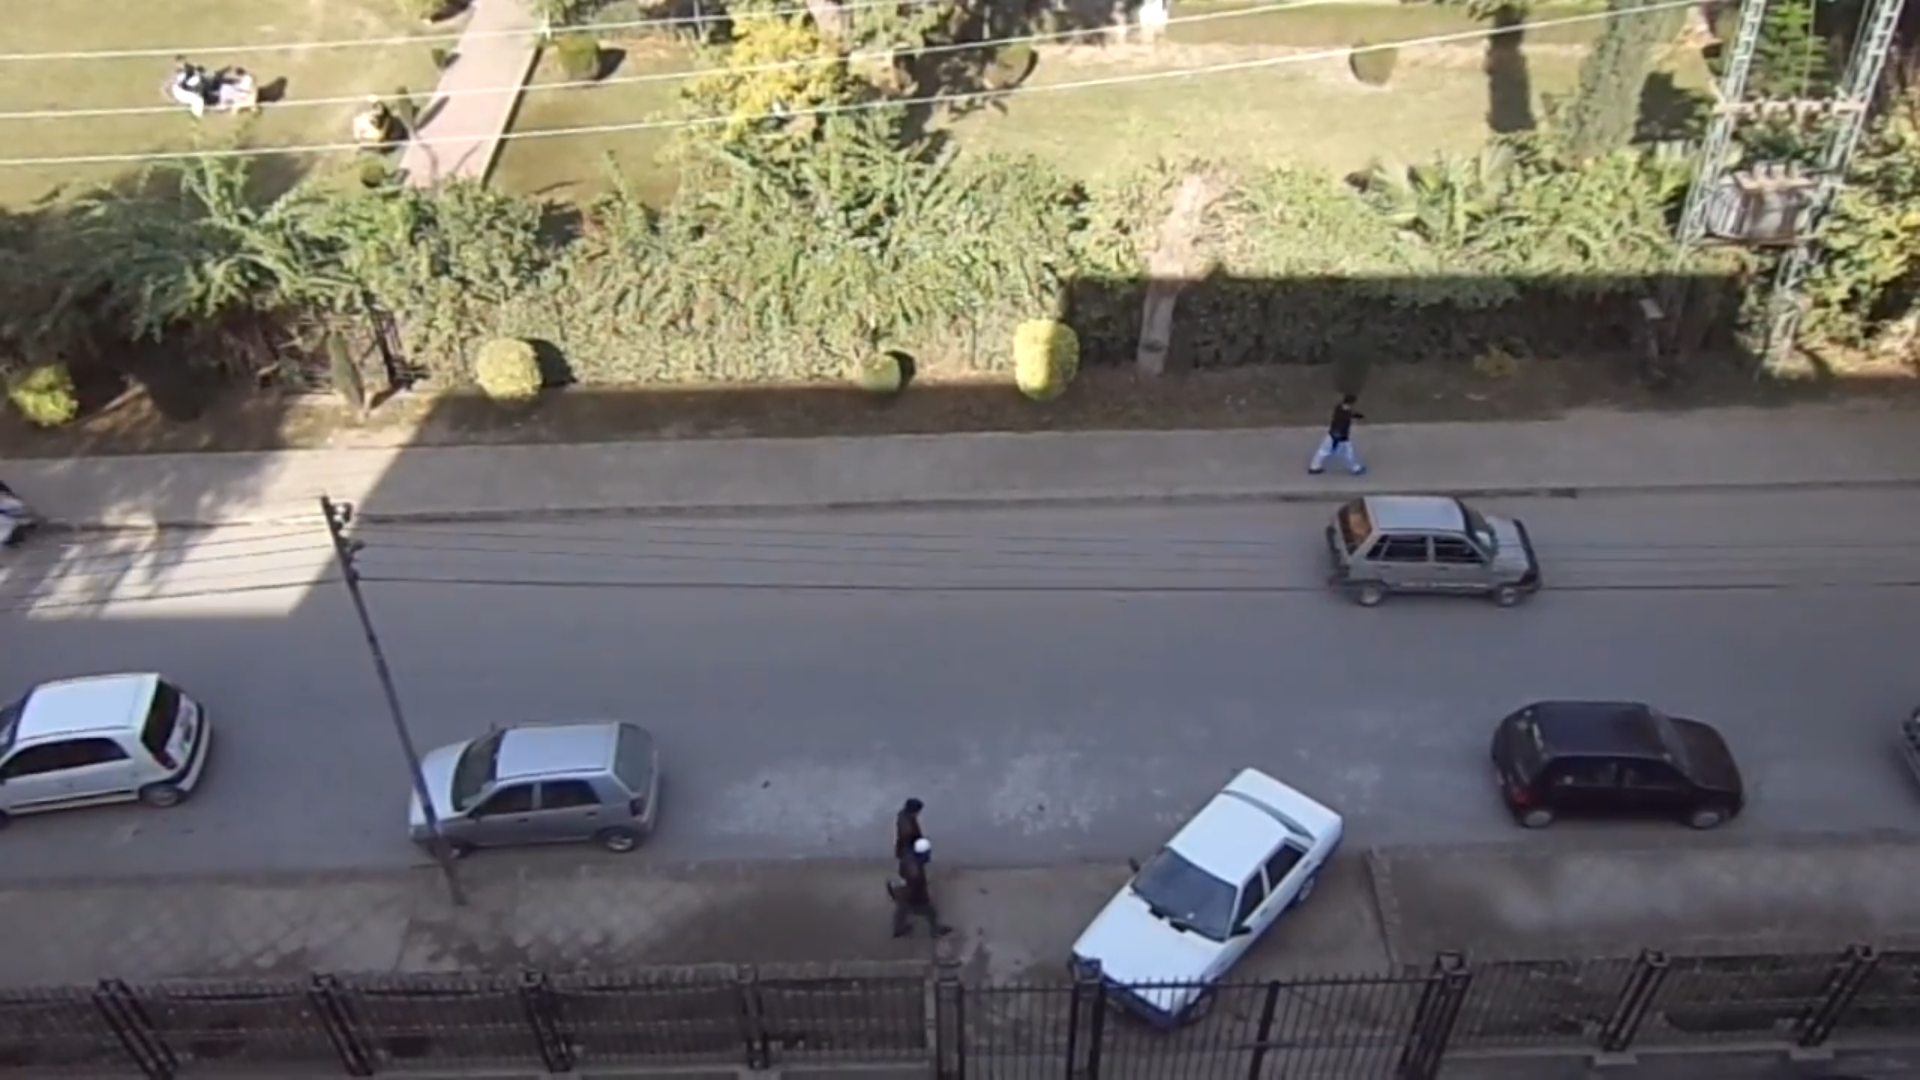
\includegraphics[width=.5\linewidth]{images/experiments/ped_humas_traffic.png}\label{fig:image1}
	}
	\subfloat[Pexels Videos 1601538.mp4]{
		\centering
		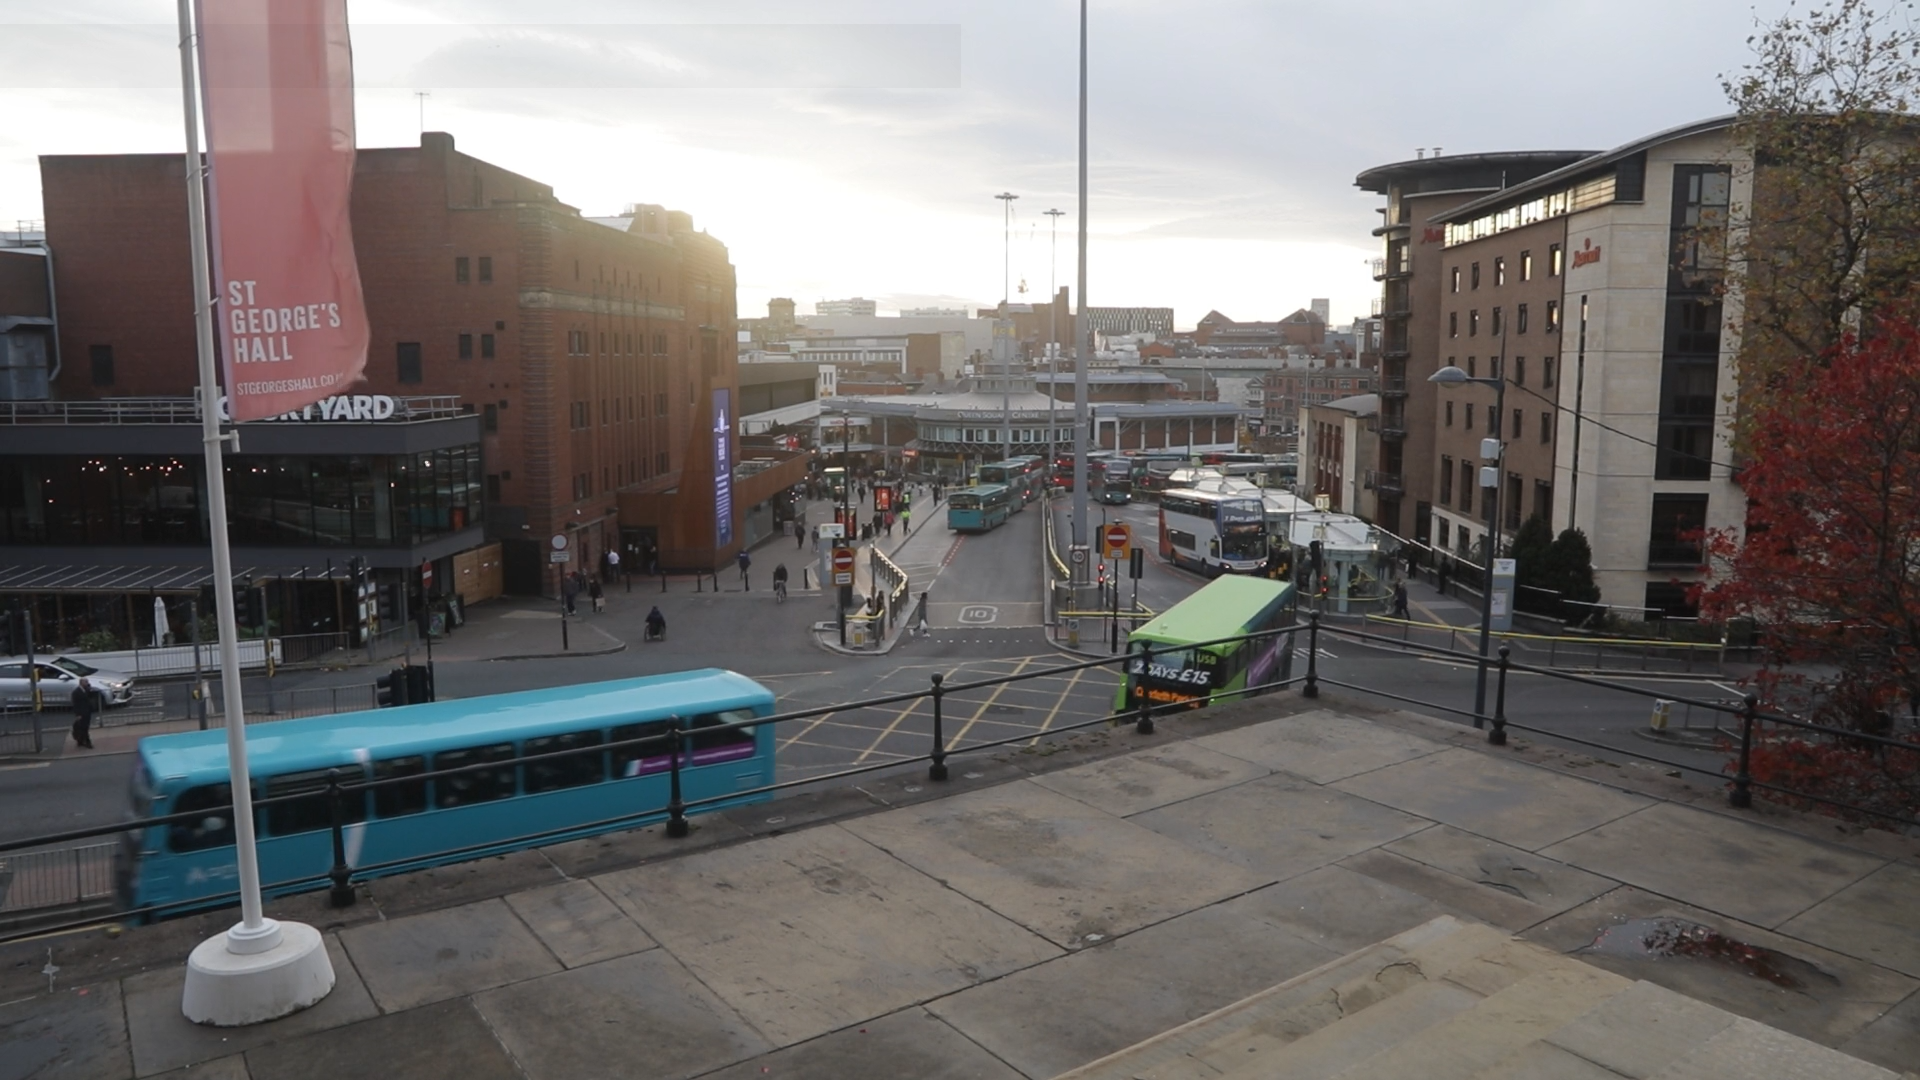
\includegraphics[width=.5\linewidth]{images/experiments/1601538.png}\label{fig:image1}
	}
	\end{figure}
	\begin{figure}
	\ContinuedFloat
	\subfloat[Pexels Videos 2577.mp4]{
		\centering
		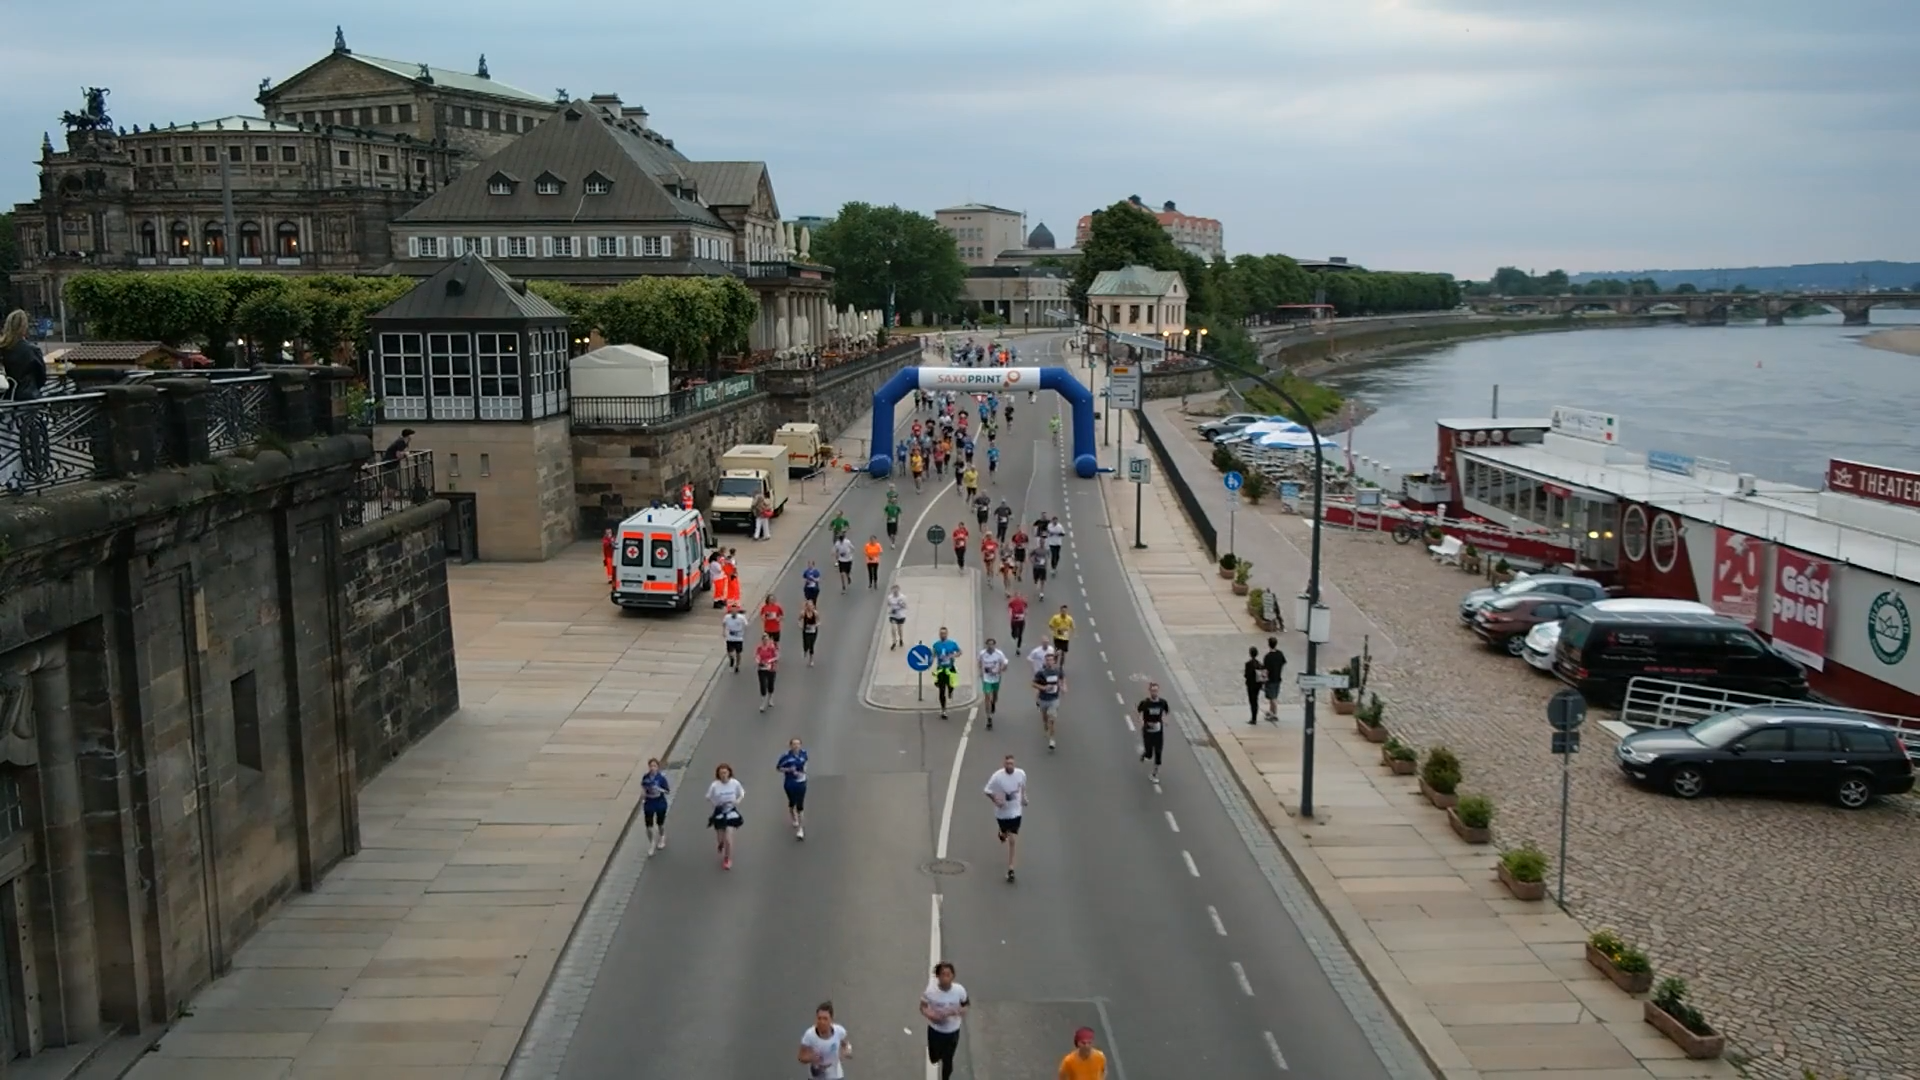
\includegraphics[width=.5\linewidth]{images/experiments/2577.png}\label{fig:image1}
	}
	\subfloat[Pexels Videos 2670.mp4]{
		\centering
		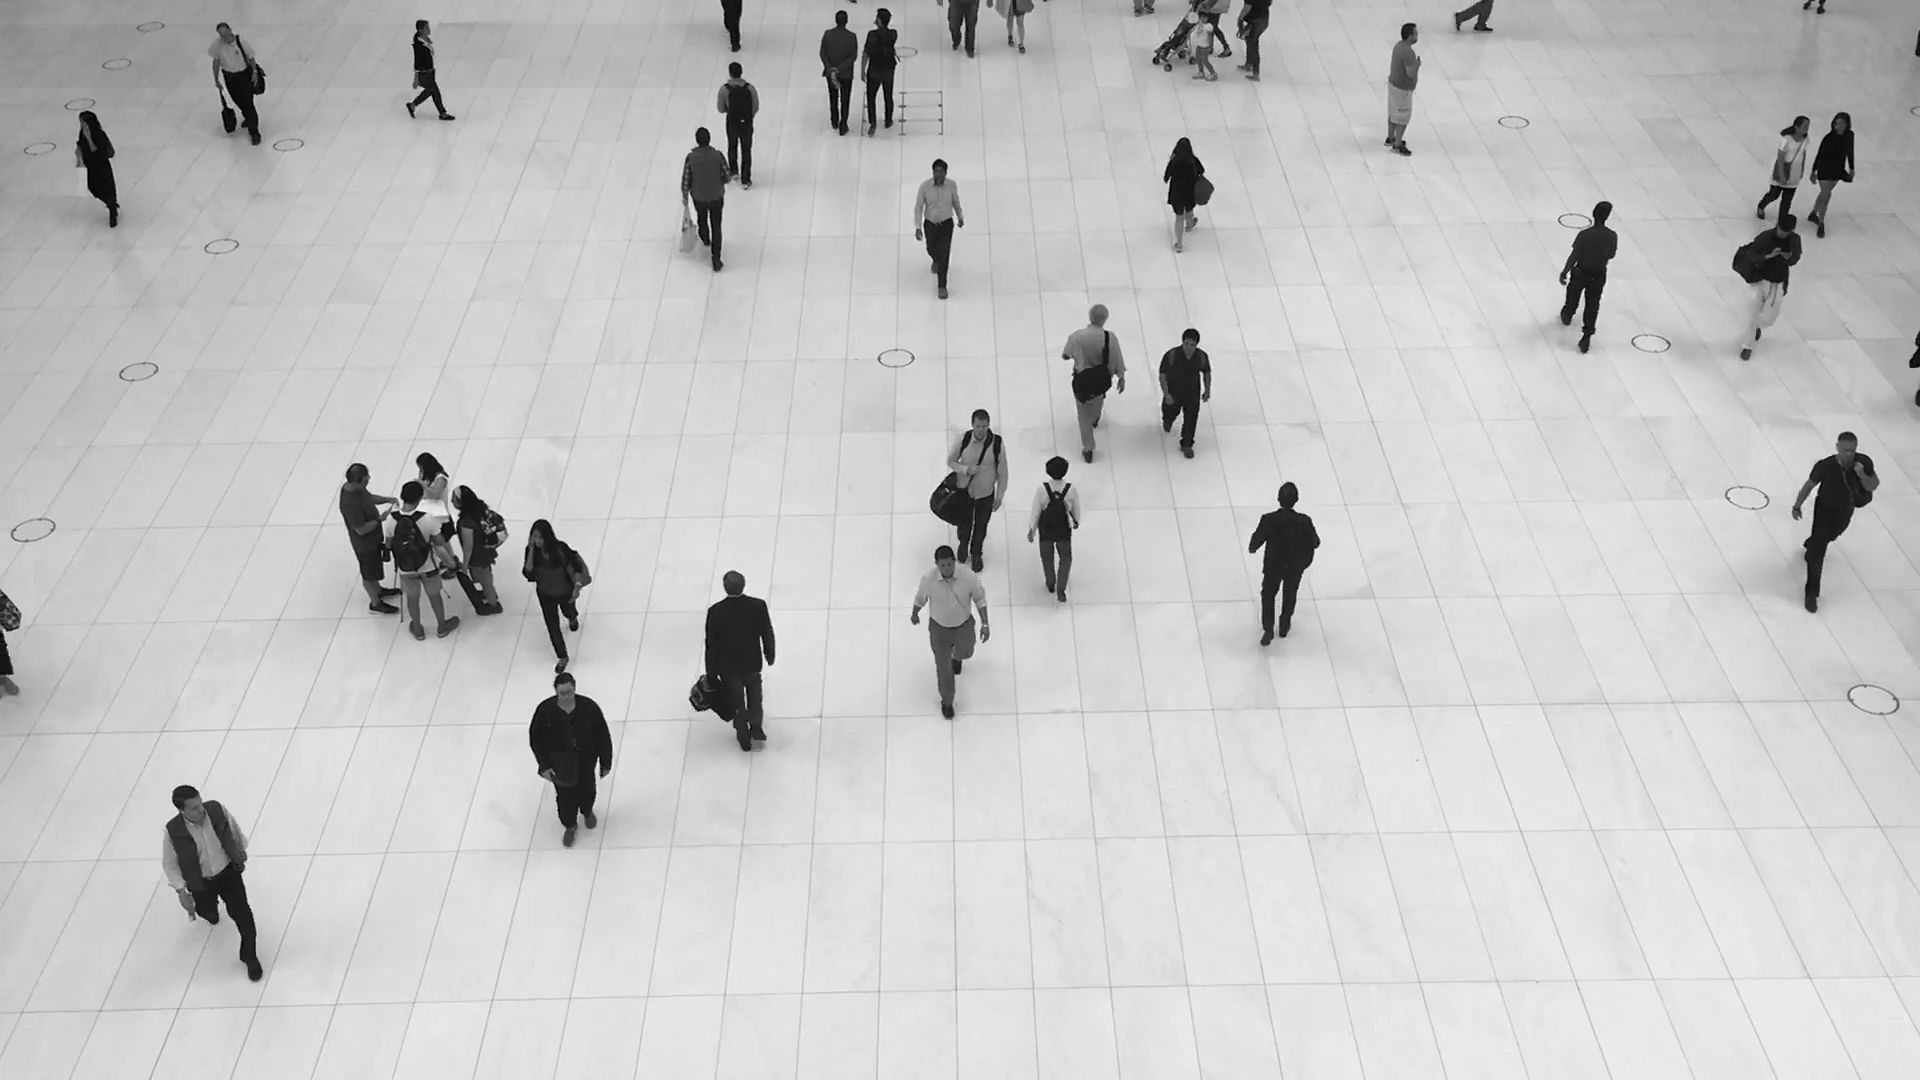
\includegraphics[width=.5\linewidth]{images/experiments/2670.png}\label{fig:image1}
	}
	\hfill
	\bigskip
	\subfloat[Pexels Videos 3047.mp4]{
		\centering
		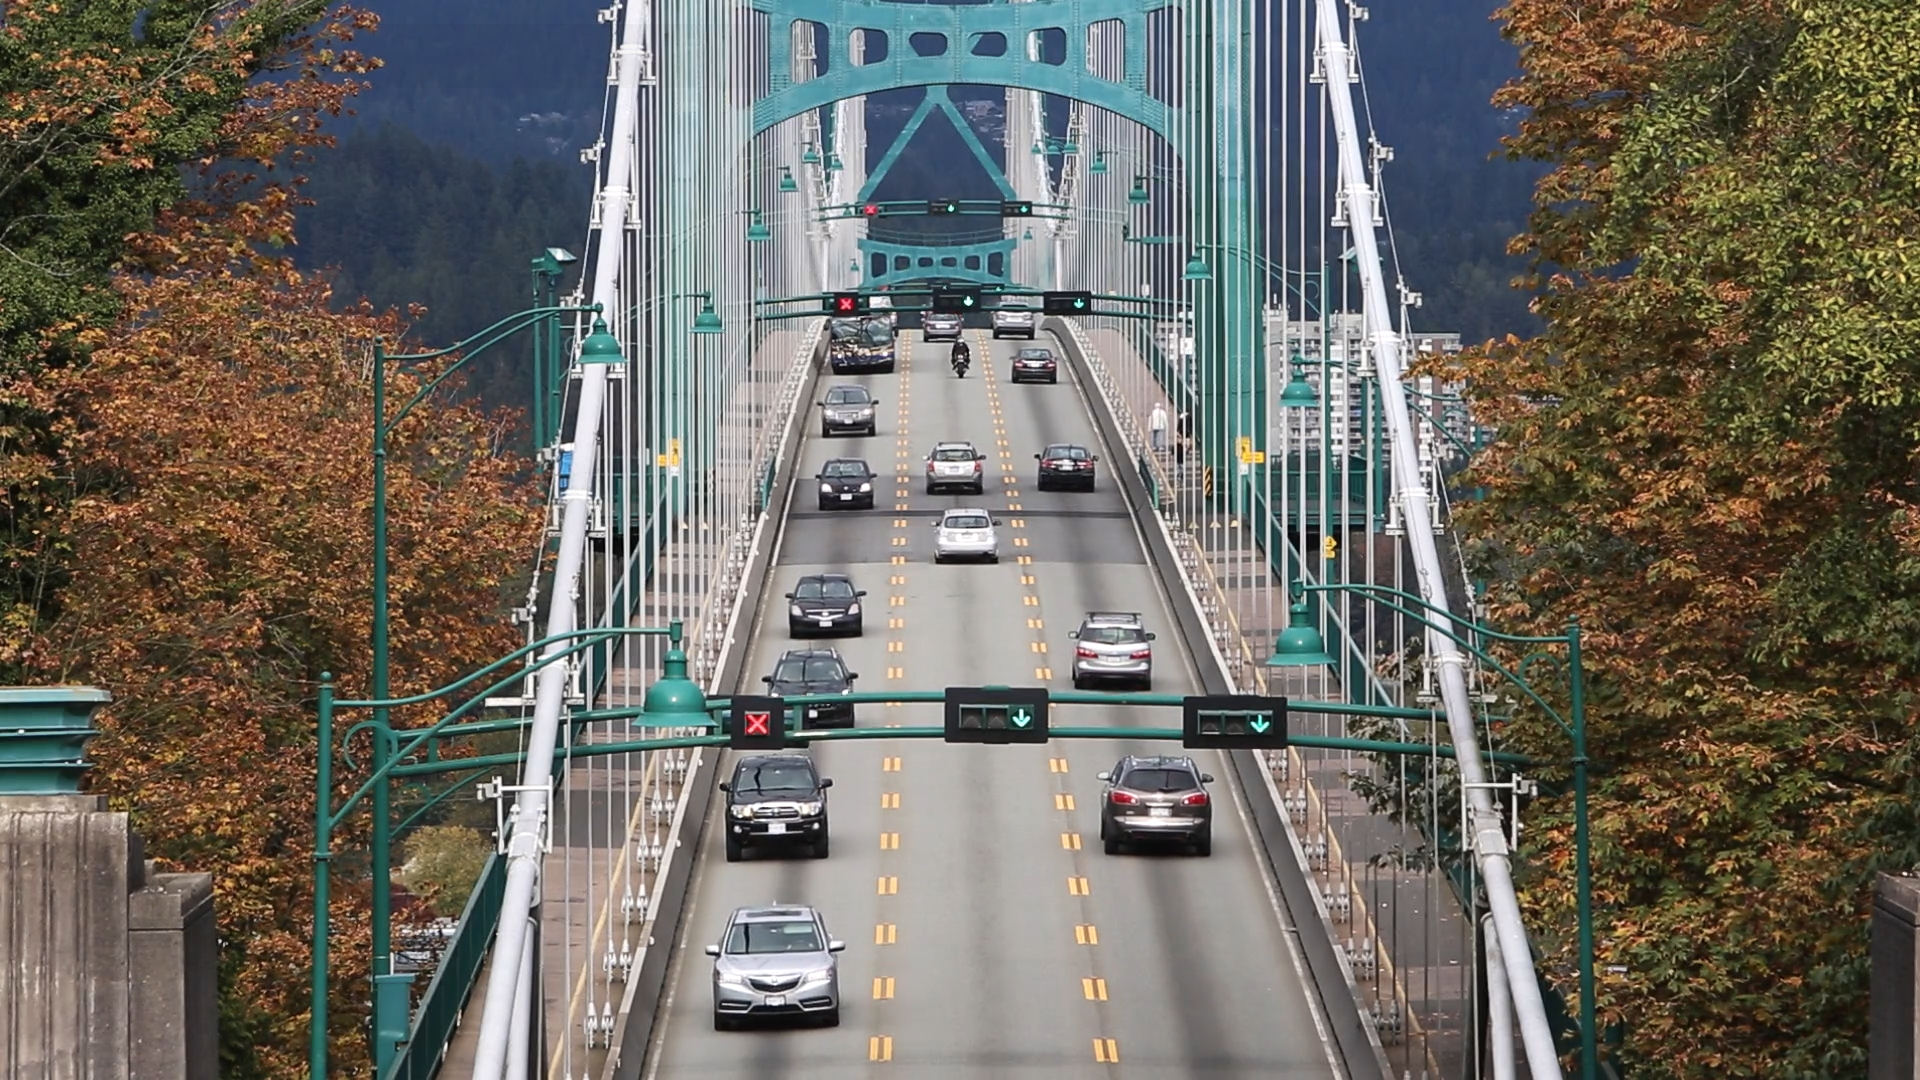
\includegraphics[width=.5\linewidth]{images/experiments/3047.png}\label{fig:image1}
	}
	\subfloat[Pexels Videos 948404.mp4]{
		\centering
		
		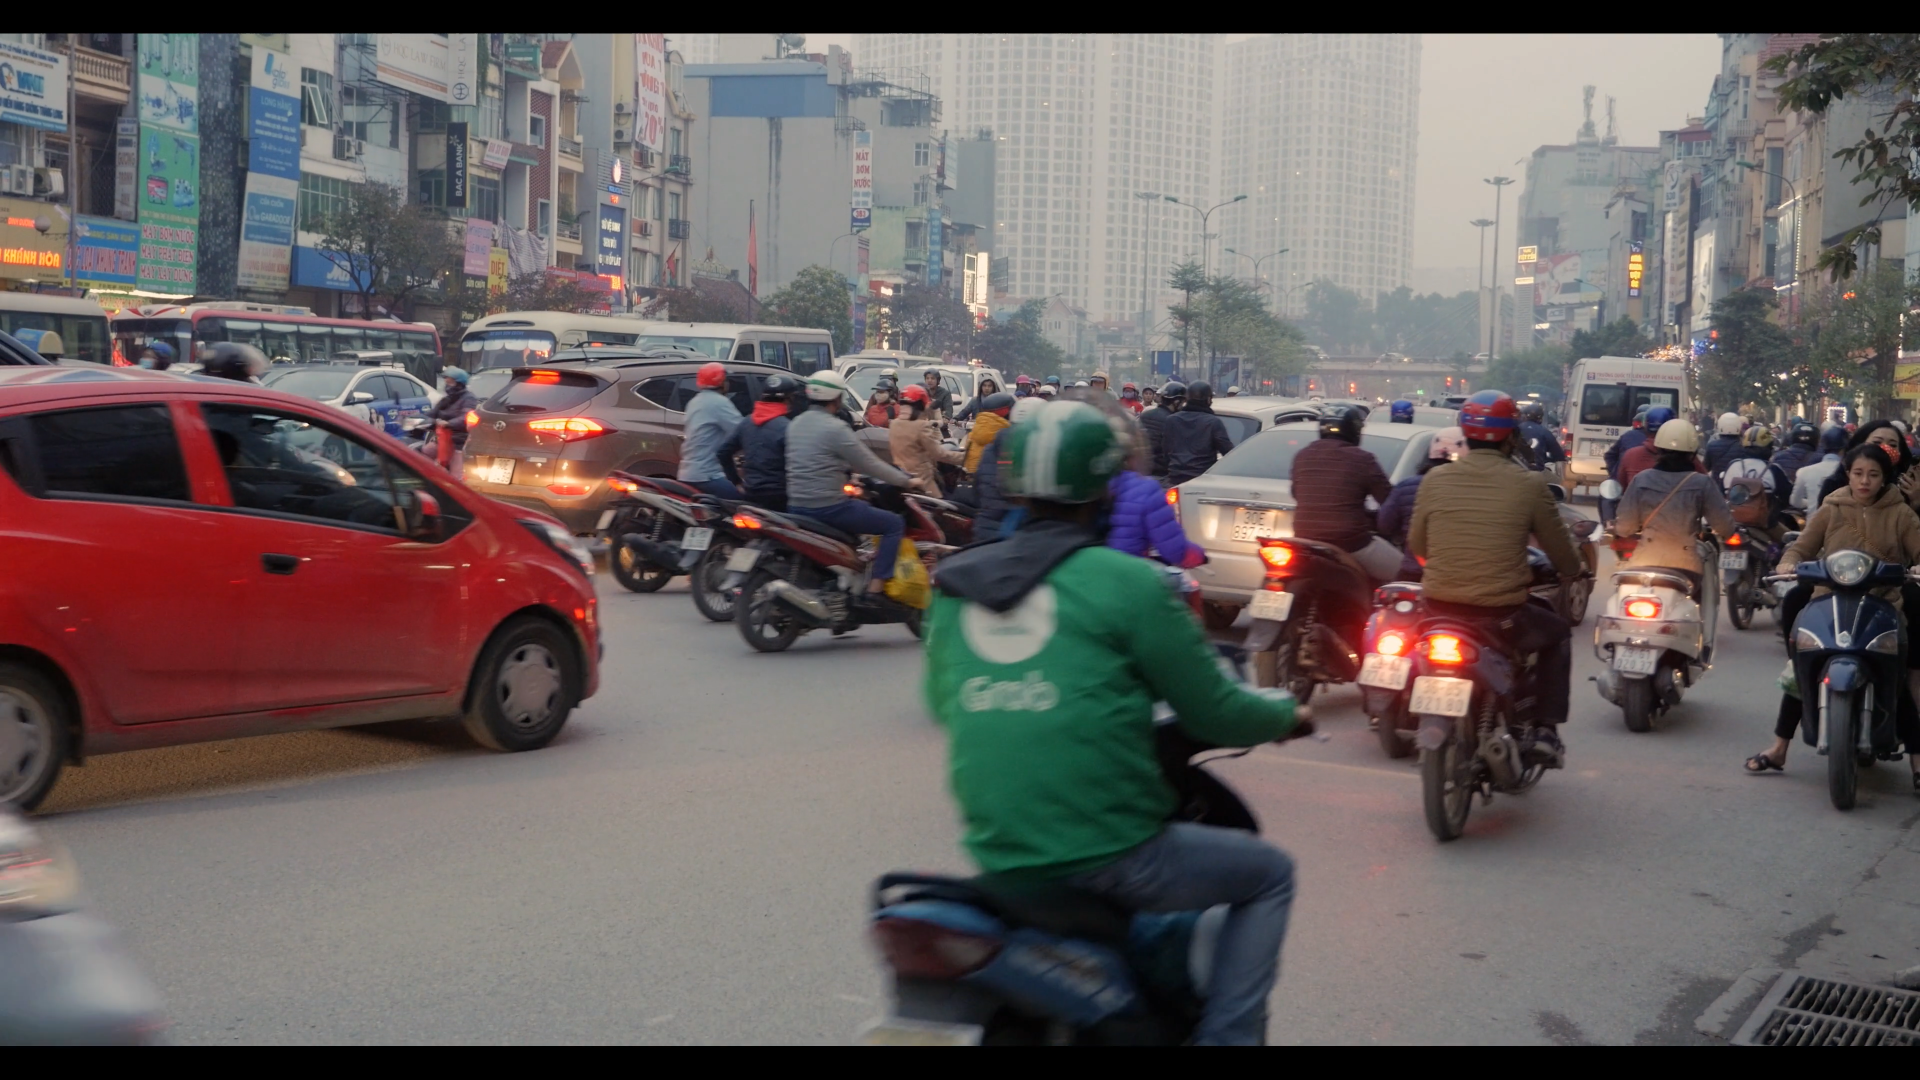
\includegraphics[width=.5\linewidth]{images/experiments/948404.png}\label{fig:image1}
	}
	\hfill
	\bigskip
	\subfloat[moderate\_traffic.mp4]{
		\centering
		
		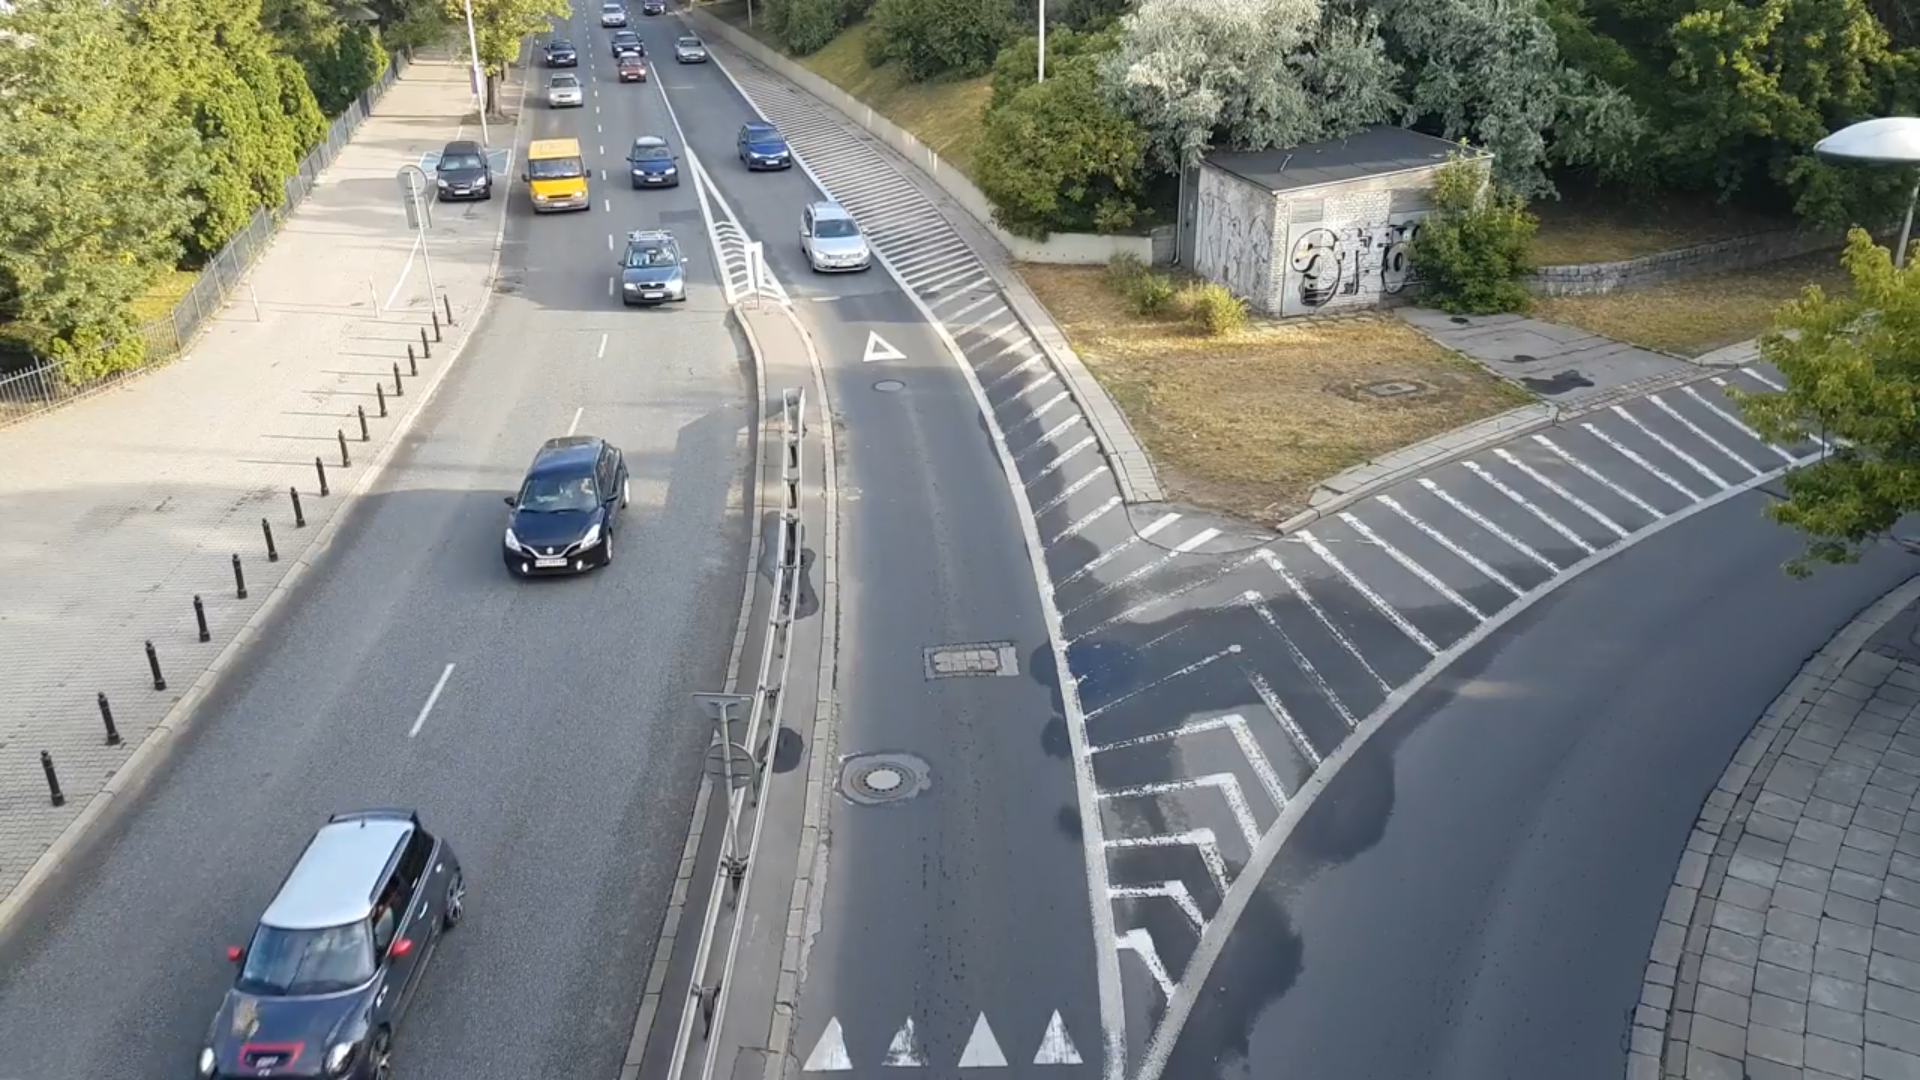
\includegraphics[width=.5\linewidth]{images/experiments/mod_traffic.png}\label{fig:image1}
	}
	\hfill
	\caption{Samples of used videos}
		\label{fig:samples}
\end{figure}
	
	
\appendix
\iffalse
\chapter{Přehled algoritmů pro vyhýbání se překážkám}
\label{obstacle_avoidance}
\begin{figure}[H]
	\caption{Souhrn algoritmů pro vyhýbání se překážkám \cite[s. 287--290]{cite:20}}
	\label{korelace}
	\subfloat{\includegraphics[width=1\textwidth]{images/6/4.png}}
	\newline
\end{figure}
\begin{figure}[H]\ContinuedFloat
		\caption{Souhrn algoritmů pro vyhýbání se překážkám \cite[s. 287--290]{cite:20}}
	\subfloat{\includegraphics[width=1\textwidth]{images/6/1.png}}
	\newline
\end{figure}
\begin{figure}[H]\ContinuedFloat
		\caption{Souhrn algoritmů pro vyhýbání se překážkám \cite[s. 287--290]{cite:20}}
	\subfloat{\includegraphics[width=1\textwidth]{images/6/2.png}}
	\newline
\end{figure}
\begin{figure}[H]\ContinuedFloat	
	\caption{Souhrn algoritmů pro vyhýbání se překážkám \cite[s. 287--290]{cite:20}}
	\subfloat{\includegraphics[width=1\textwidth]{images/6/3.png}}
	\newline
\end{figure}
\fi
\printindex

\bibliographystyle{unsrt}
\bibliography{ctutest}


\end{document}
